\documentclass[9pt]{report}

\usepackage{talk}
\usepackage{mathpazo}
\renewcommand{\baselinestretch}{1.05}
% \usepackage[export]{adjustbox}

\newcommand{\draw}[2]{#1^{(#2)}}
\newcommand{\displayfrac}[2]{{\displaystyle \frac{\displaystyle #1}{\displaystyle #2}}}
\newcommand{\simvar}[1]{#1^{\textrm{sim}}}
\newcommand{\simdraw}[2]{#1^{\textrm{sim}(#2)}}

\begin{document}
\sf%
\mbox{ }
\\[12pt]
\spc{\Large\bfseries \myemph{SARS-CoV-2 PCR diagnostic testing:}}
\\[4pt]
\spc{\Large\bfseries \myemph{test site variation and time trends}}
\\[36pt]
\noindent
\spc{\bfseries \myemph{Bob Carpenter}}
\\[2pt]
\spc{Center for Computational Mathematics}
\\[2pt]
\spc{Flatiron Institute}
\vfill
\noindent
\spc{\small \myemph{@ Paris Diderot / INSERM}} \hfill

\includegraphics[height=24pt]{img/flatiron-logo.png}
\hfill

\includegraphics[height=24pt]{img/stan-logo.png}

\sld{SARS-CoV-2 test accuracy varies}

\begin{itemize}
\item by testing \myemph{site}
\item by \myemph{time} since infection
\item by \myemph{test type} (PCR vs. lateral flow)
\item and presumably by \myemph{variant} (alpha, delta, omicron, $\ldots$)
\end{itemize}

\sld{Sensitivity and specificity}
\begin{itemize}
\item \myemph{sensitivity} is accuracy on positive cases
\item \myemph{specificity} is accuracy on negative cases
\item if $Z_n$ is disease status for subject $n$ and $Y_n$ is test result,
  \begin{subitemize}
  \item $\textsf{sensitivity} = \textrm{Pr}[Y_n = 1 \mid Z_n = 1]$
  \item $\textsf{specificity} = \textrm{Pr}[Y_n = 0 \mid Z_n = 0]$
  \end{subitemize}
\end{itemize}

\sld{Diagnosis \& calibration}
\begin{itemize}
\item for \myemph{diagnostic testing},
  \begin{subitemize}
  \item test result $Y_n$ is \myemph{observed}, but
  \item disease status $Z_n$ is \myemph{latent}
  \end{subitemize}
\item for \myemph{calibration testing},
  \begin{subitemize}
  \item test result \myemph{and} disease status are \myemph{observed}
  \item \myemph{known negatives} use pre-Covid blood samples
  \item \myemph{known positives} are independently verified cases
  \end{subitemize}
\end{itemize}

\sld{Population prevalence}
\begin{itemize}
\item \myemph{prevalence} is proportion of population who are
  positive
\item we use $\pi \in [0, 1]$ for prevalence
\item \myemph{prevalence varies} by the following (among other things!)
  \begin{subitemize}
    \vspace*{-12pt}
  \item time 
  \item location
  \item age
  \item sex
  \item socio-economic status (income quintile or decile)
  \item ethnicity (very ad hoc by country)
  \item intervention (lockdown, masks, distancing, etc.)
  \end{subitemize}
\end{itemize}
  
\sld{Inferential goals}
\begin{itemize}
\item we have three goals in modeling diagnostic tests
  \begin{subitemize}
  \item estimate \myemph{diagnostic accuracy}: $\textrm{Pr}[Y_n \mid Z_n])$
  \item estimate \myemph{population prevalence}: $p(\pi \mid Y, Z)$
  \item provide probabilistic \myemph{diagnostics}: $\textrm{Pr}[Y_n = 1 | Z_n]$
  \end{subitemize}
\end{itemize}

\sld{Bayesian modeling}
\begin{itemize}
\item Andrew Gelman says \myemph{Donald Rubin advises}:
  \begin{subitemize}
  \item model what we'd do if we \myemph{had all the data},
  \item then \myemph{turn the Bayesian crank} to infer unknowns
  \end{subitemize}
\item This allows us to design models without
  \begin{subitemize}
  \item worrying about the \myemph{details of inference}
  \item deciding a priori how to handle \myemph{``missing'' data}
  \end{subitemize}
\end{itemize}

\sld{Model basics for site variation}
\begin{itemize}
\item diagnostic tests known to \myemph{vary by test site}
\item we will build up to a model where
  \begin{subitemize}
  \item \myemph{likelihood}: sensitivity and specificity vary by site
    and individuals are \myemph{exchangeable}
  \item \myemph{prior}: hierarchical population model of site sensitivity and specificity
  \end{subitemize}
\item we will \myemph{observe}
  \begin{subitemize}
  \item \myemph{test site and result} for each individual
  \item \myemph{disease status} fo some individuals
  \end{subitemize}
\end{itemize}

\sld{Variable notation}
\begin{itemize}
  \item \myemph{parameters}
  \begin{subitemize}
  \item $\pi \in (0, 1)$: \myemph{prevalence} of infection in population
  \item $\theta_{k, 1}$: \myemph{sensitivity} at test site $k \in 1:K$
  \item $\theta_{k, 0}$: \myemph{specificity} at test site $k \in 1:K$
  \end{subitemize}
\item \myemph{data} (both observed and \myemph{``missing''}
  \begin{subitemize}
  \item $N$ total test \myemph{subjects}
  \item $y_n \in \{ 0, 1 \}$: \myemph{test result}
  \item $z_n \in \{ 0, 1 \}$: \myemph{disease status} of subject $n$
  \item $kk_n \in 1{:}K$: \myemph{site} for test $n$
  \item $y_n \in \{ 0, 1 \}$: \myemph{test result} for individual $n$
  \end{subitemize}
\end{itemize}

\sld{Start without site variation}
\begin{itemize}
\item start with simple model, then criticize and revise
  \begin{subitemize}
  \item baseline model from \myemph{Bendavid et al.} (2020)
    \end{subitemize}
\item assume sensitivity and specificity \myemph{do not vary} by
  site
\item two views on lack of variation
  \begin{subitemize}
  \item \myemph{choice of prior}: (e.g., $\theta_{i, k} = \theta_{i, k'}$), or
  \item \myemph{choice of likelihood}: one parameter each for sensitivity
    \& specificity
  \end{subitemize}
\end{itemize}

\sld{Simple non-varying model}

\begin{itemize}
\item let $\theta_1$ be \myemph{sensitivity} and $\theta_0$ \myemph{specificity}
\item uniform \myemph{priors} on probabilities
  \begin{subitemize}
  \item $\pi, \ \theta_1, \ \theta_0 \sim \textrm{uniform}(0, 1)$
  \item equivalently, standard logistic prior on log odds
  \end{subitemize}
\item \myemph{``complete'' data likelihood} for missing \& non-missing
  \begin{subitemize}
  \item $z_n \sim \textrm{bernoulli}(\pi)$
  \item $y_n \sim
    \begin{cases}
      \textrm{bernoulli}(\theta_1) & \textsf{if } z_n = 1
      \\
      \textrm{bernoulli}(1 - \theta_0) & \textrm{if } z_n = 0
    \end{cases}$
  \end{subitemize}
\item \myemph{calibration} cases have observed $z_n$
\end{itemize}

\sld{Data and fit for simple model}
\begin{subitemize}
\item \myemph{positive calibration} ($z_n = 1$): 103 / 122
\item \myemph{negative calibration} ($z_n = 0$) : 399 / 401
\item \myemph{missing disease status} ($z_n$ unknown): 50 / 3300
\end{subitemize}
\vspace*{-6pt}
\begin{center}
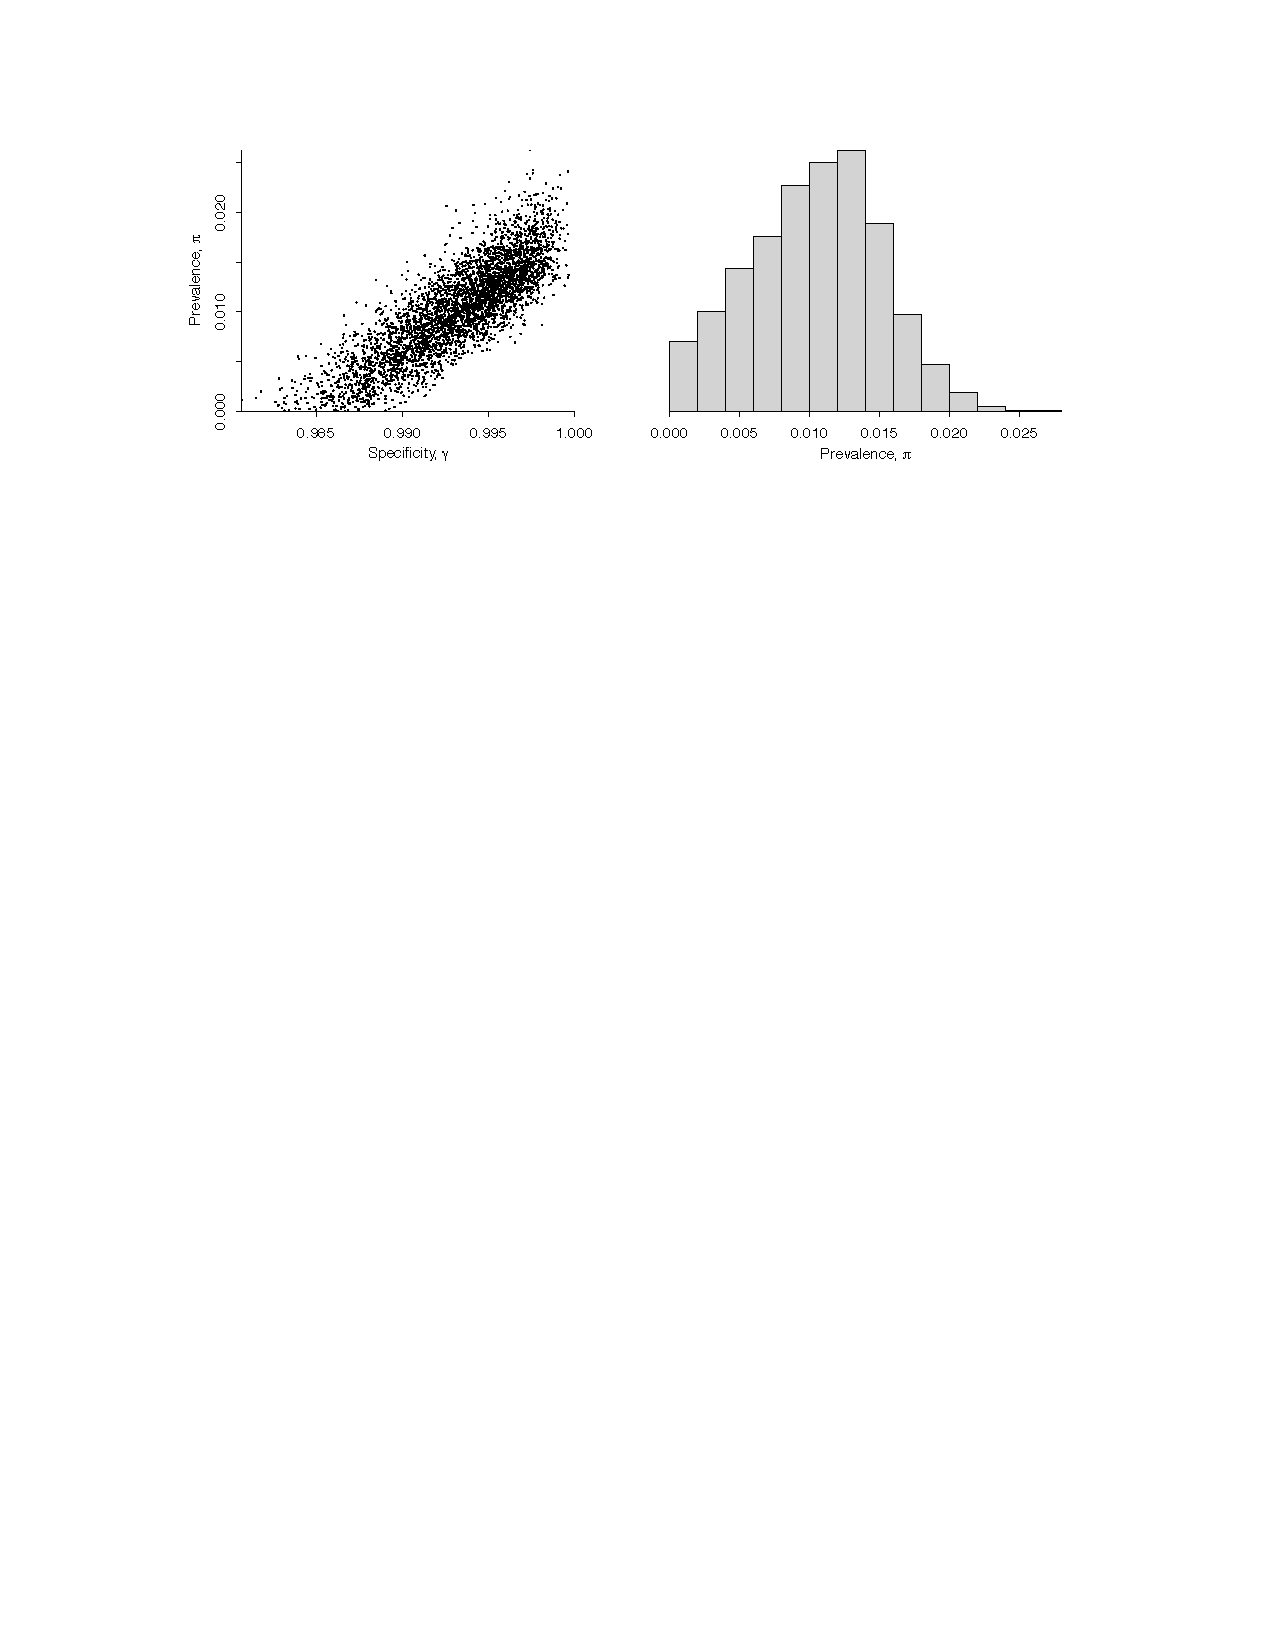
\includegraphics[width=0.9\textwidth]{img/simple-inf.pdf}
\end{center}
\vspace*{-8pt}
\begin{subitemize}
\item 95\% \myemph{shortest posterior interval} (0, 1.8\%) for $\pi$ \myemph{inconclusive}
\end{subitemize}

\sld{Hierarchical model}
\begin{itemize}
  \item \myemph{hierarchical priors} for sensitivity and specificity
\begin{subitemize}
\item \myemph{specificity}: $\textrm{logit}(\theta_{k, 0}) \sim \textrm{normal}(\mu_0, 
  \sigma_0)$
\item \myemph{sensitivity}: $\textrm{logit}(\theta_{k, 1}) \sim \textrm{normal}(\mu_1, 
  \sigma_1)$
\end{subitemize}
\item \myemph{hyperpriors} for hierarchical parameters
  \begin{subitemize}
  \item hyperprior mean: $\mu_0, \mu_1 \sim \textrm{normal}(2, 4)$
  \item hyperprior scale (specificity): $\sigma_0 \sim \textrm{normal}_+(0, \tau_0)$
  \item hyperprior scale (sensitivity): $\sigma_1 \sim
    \textrm{normal}_+(0, \tau_1)$
  \end{subitemize}
\item we evaluate \myemph{broad} and \myemph{weakly
    informative} priors
  \begin{subitemize}
  \item weakly informative set \myemph{expected scale} and \myemph{regularize}
  \end{subitemize}
\end{itemize}


\sld{Multivariate hierarchical model}
\begin{itemize}
  \item sensitivity and specificity are \myemph{correlated}
    \begin{subitemize}
    \item \myemph{positively} due to care taken by lab
    \item \myemph{negatively} based on decision threshold
    \end{subitemize}
  \item we'd like to impose a \myemph{multivariate prior}
  $$\begin{bmatrix} \theta_{0, k} & \theta_{1, k} \end{bmatrix}
  \sim \textrm{multi-normal}(\mu, \Omega)$$
  \vspace*{-12pt}
  \begin{subitemize}
    \item but no sites in our data have \myemph{positive {\slshape and}\ negative}
      calibration tests
    \end{subitemize}
\end{itemize}
  
\sld{Inferences from hierarchical model}
\vspace*{-12pt}
\begin{subitemize}
  \item site $k = 1$ has diagnostic tests with \myemph{unknown disease
      status}
    \vspace*{-4pt}
  \item yielding estimates for \myemph{population prevalence} and
    \vspace*{-4pt}
  \item estimates for \myemph{test accuracy} at a \myemph{site with no calibration data}
\end{subitemize}
\qquad 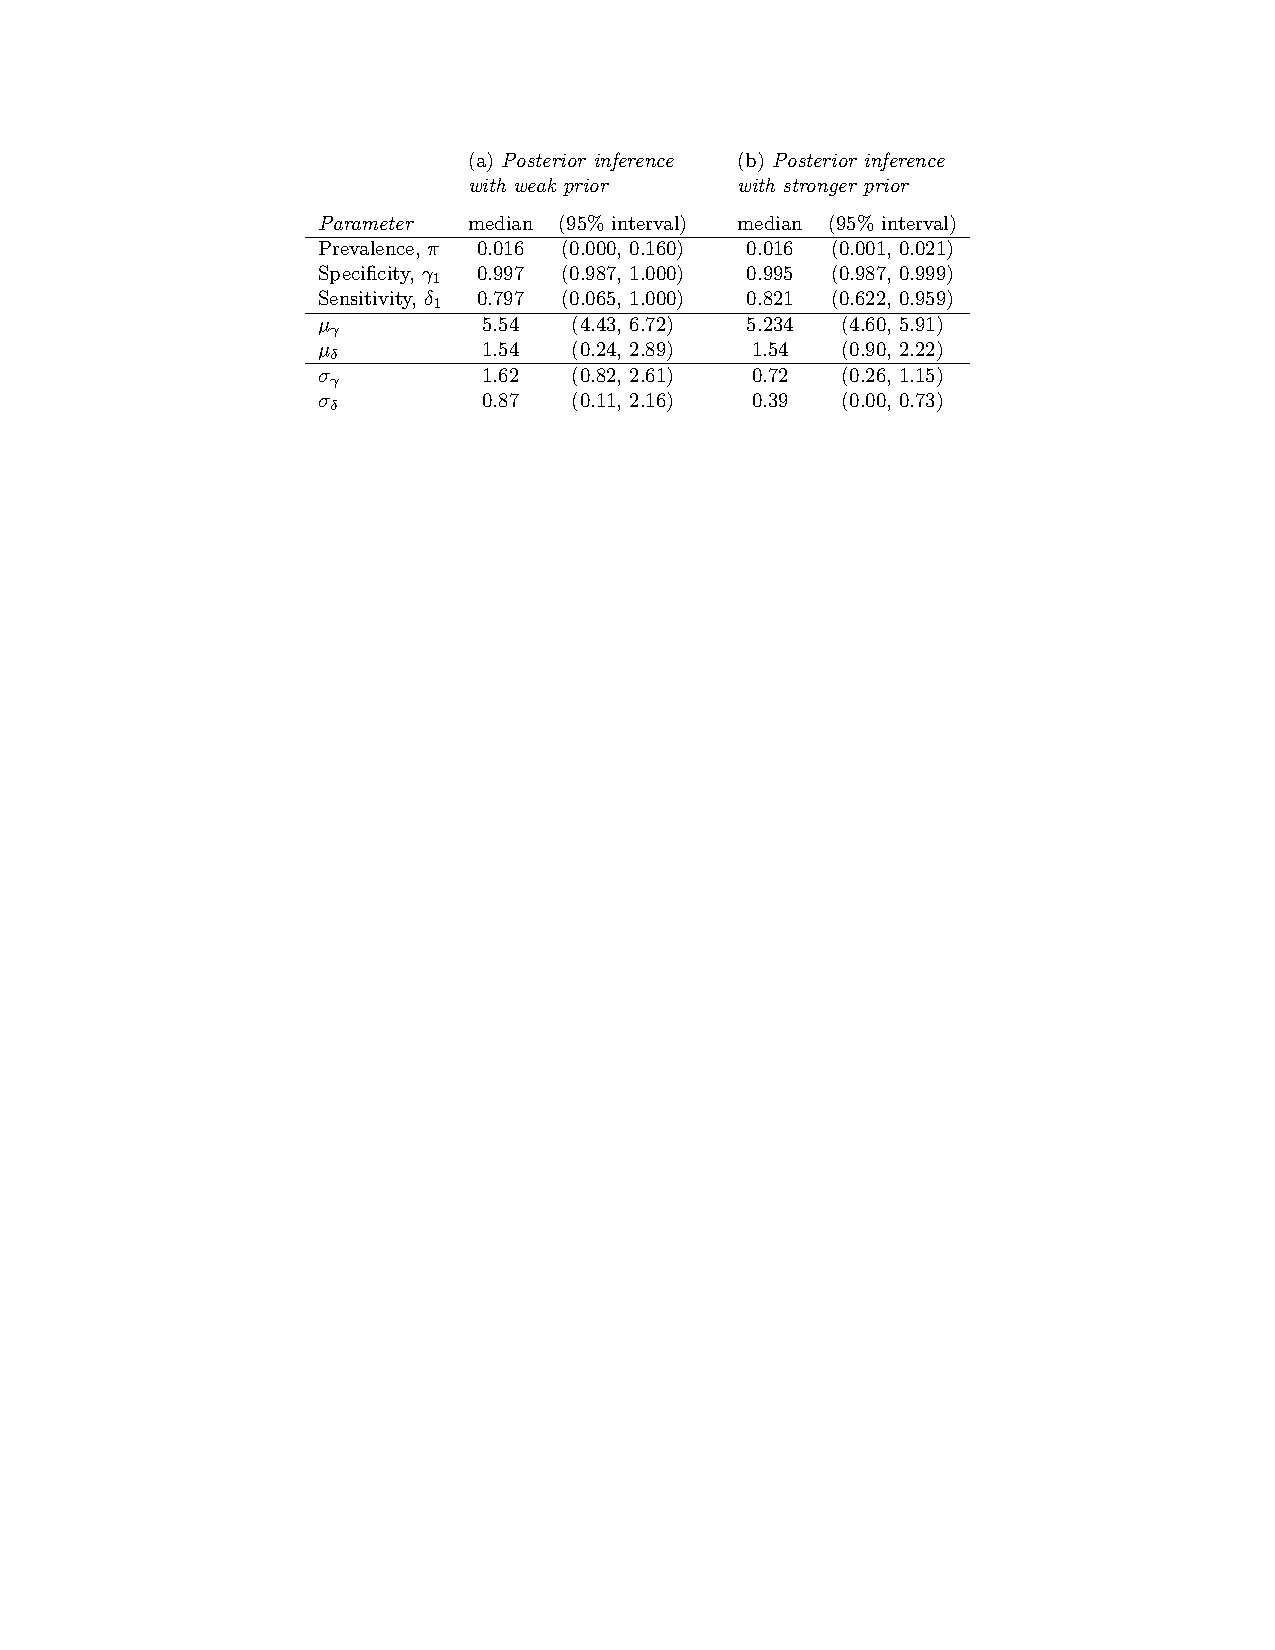
\includegraphics[width=0.9\textwidth]{img/results-table.pdf}
\vfill

\sld{Sensitivity analysis}
\begin{subitemize}
  \item \myemph{sensitivity analysis} varies hyperparameter scales $\tau_0,
    \tau_1$
    \vspace*{-6pt}
  \item \myemph{boxes $\tau_1$}:  sensitivity hyperprior in (0.01, 0.25, 0.5, 0.75, 1)
    \vspace*{-6pt}
  \item \myemph{horizontal axis $\tau_0$}: specificity hyperprior (0--1)
    \vspace*{-6pt}
  \item \myemph{vertical axis $\pi$}:  est.\ median \& central 90\% prevalence
  \end{subitemize}
\quad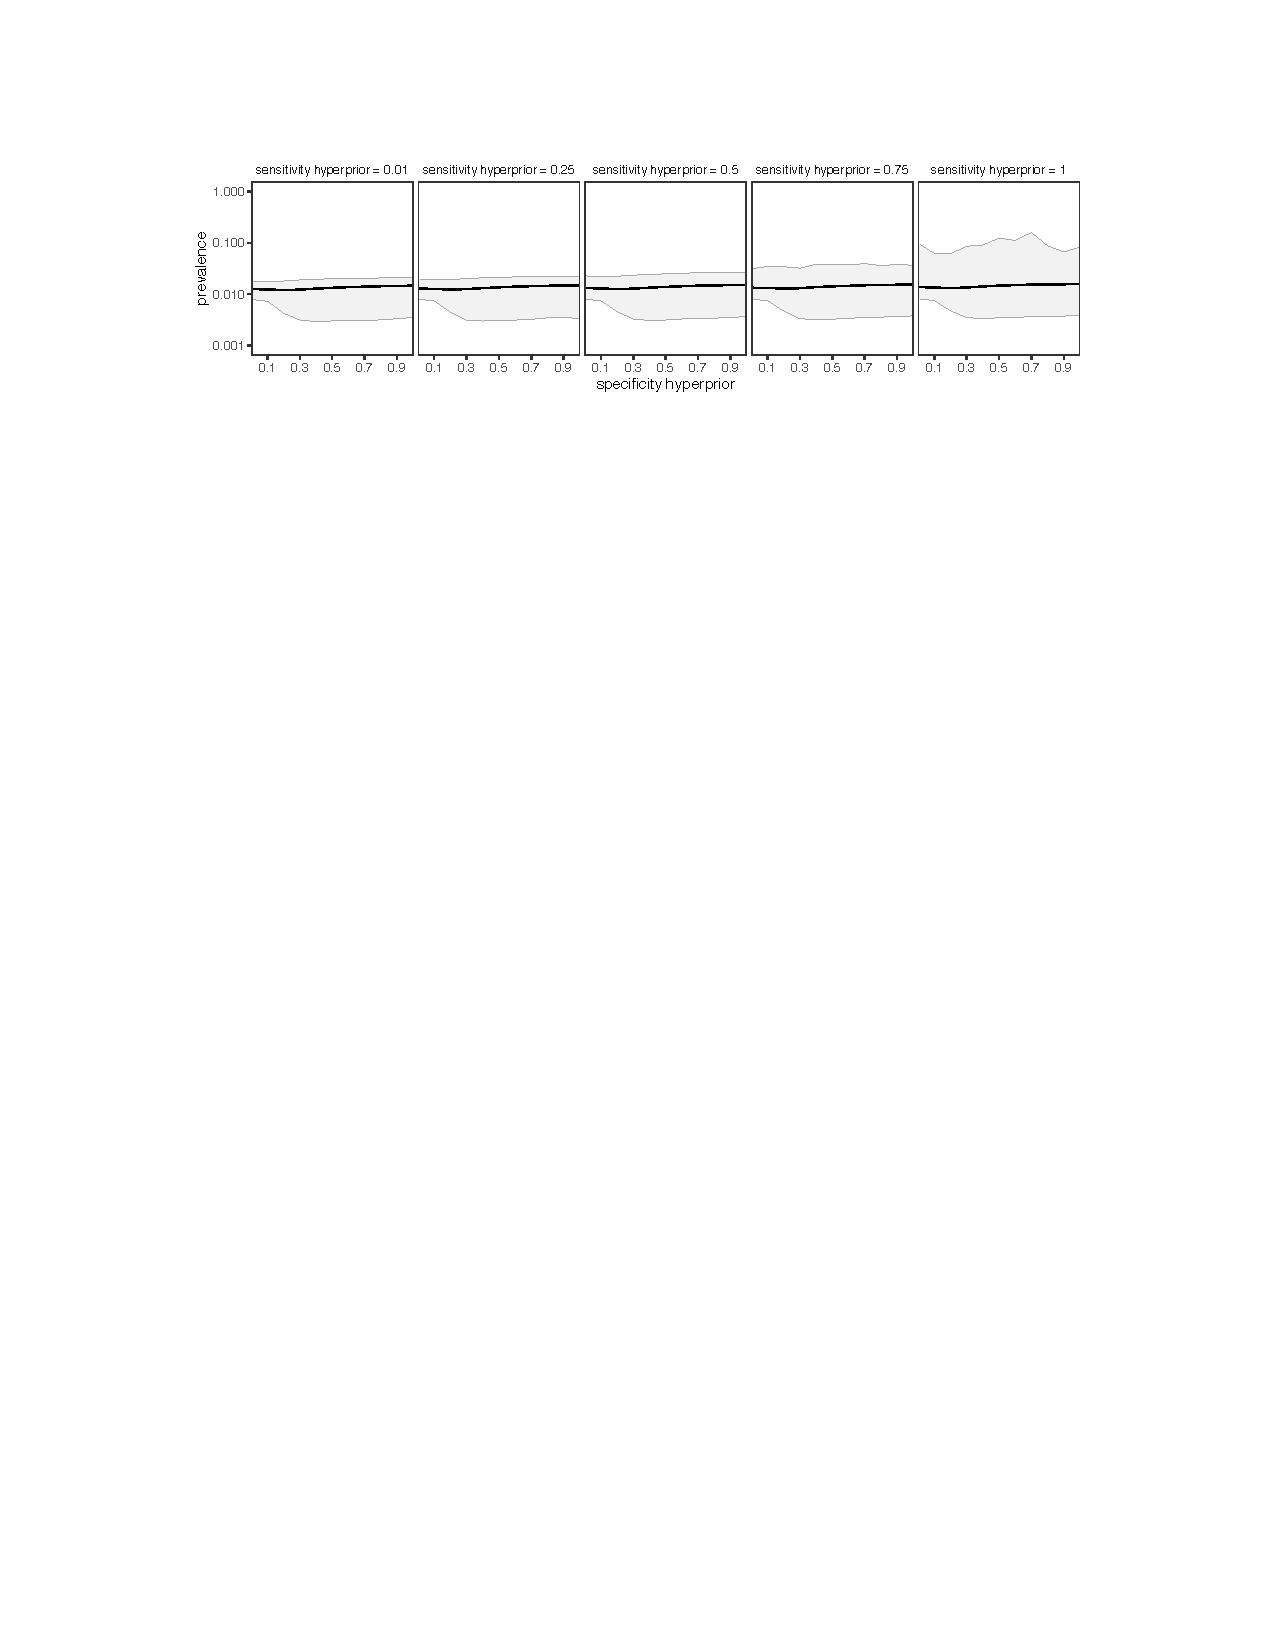
\includegraphics[width=1.05\textwidth]{img/sensitivity-analysis.pdf}    
\begin{subitemize}
  \item prevalence estimate \myemph{not very sensitive} to hyperparameter scale
  \end{subitemize}

\sld{Poststratification}
\begin{itemize}
\item our paper discusses applying \myemph{poststratification} to
  \begin{subitemize}
  \item \myemph{adjust} for differences between \myemph{sample and population}
  \end{subitemize}
\item idea is to let \myemph{prevalence vary} by
  \begin{subitemize}
  \item sex
  \item age
  \item ethnicity 
  \item region plus regional predictor (e.g., avg.~income)
  \end{subitemize}
\item Bendavid et al. poststratified, but didn't share covariates
\item we poststratified UK (\& Indiana), but no time to present
\end{itemize}

\sld{Implementation}
\begin{itemize}
\item we coded our models in \myemph{Stan} (paper appendix, GitHub)
\item Stan has \myemph{continuous parameters}, so we
  \begin{subitemize}
  \item \myemph{marginalize} discrete ``missing data'' (disease status
    $z_n$)
  \end{subitemize}
\item \myemph{complete data likelihood}:
  {\small
  \begin{eqnarray*}
    p(y_n, z_n \mid \pi, \theta)
    & = & \textrm{bernoulli}(z_n \mid \pi)
          \\
    & \times & \textrm{bernoulli}\big(y_n \mid \textrm{ifelse}(z_n,
        \ \  \theta_{1,
      \, kk[n]},  \ \ 1 - \theta_{0, \, kk[n]})\big)
  \end{eqnarray*}}
\item \myemph{likelihood}:
  $$\textrm{Pr}\left[y_n = 1 \mid \pi, \theta\right]
    = \underbrace{\pi \cdot \theta_{1, \, kk[n]}}_{\textrm{true
        positive rate}}
    + \underbrace{(1 - \pi) \cdot (1 - \theta_{0, \,
        kk[n]})}_{\textrm{false negative rate}}$$
\end{itemize}


\sld{Sensitivity growth and decay}
\begin{itemize}
\item at time of \myemph{infection}: viral load/test sensitivity is \myemph{zero}
\item at time of \myemph{symptom onset}: they are \myemph{maximized}
\item \myemph{after onset}: clearance for \myemph{exponential decay}
  \vfill
\item assuming a fixed sensitivity produces a kind of \myemph{average}
\end{itemize}

\sld{Raw data: {\slshape hospitalized patients}}

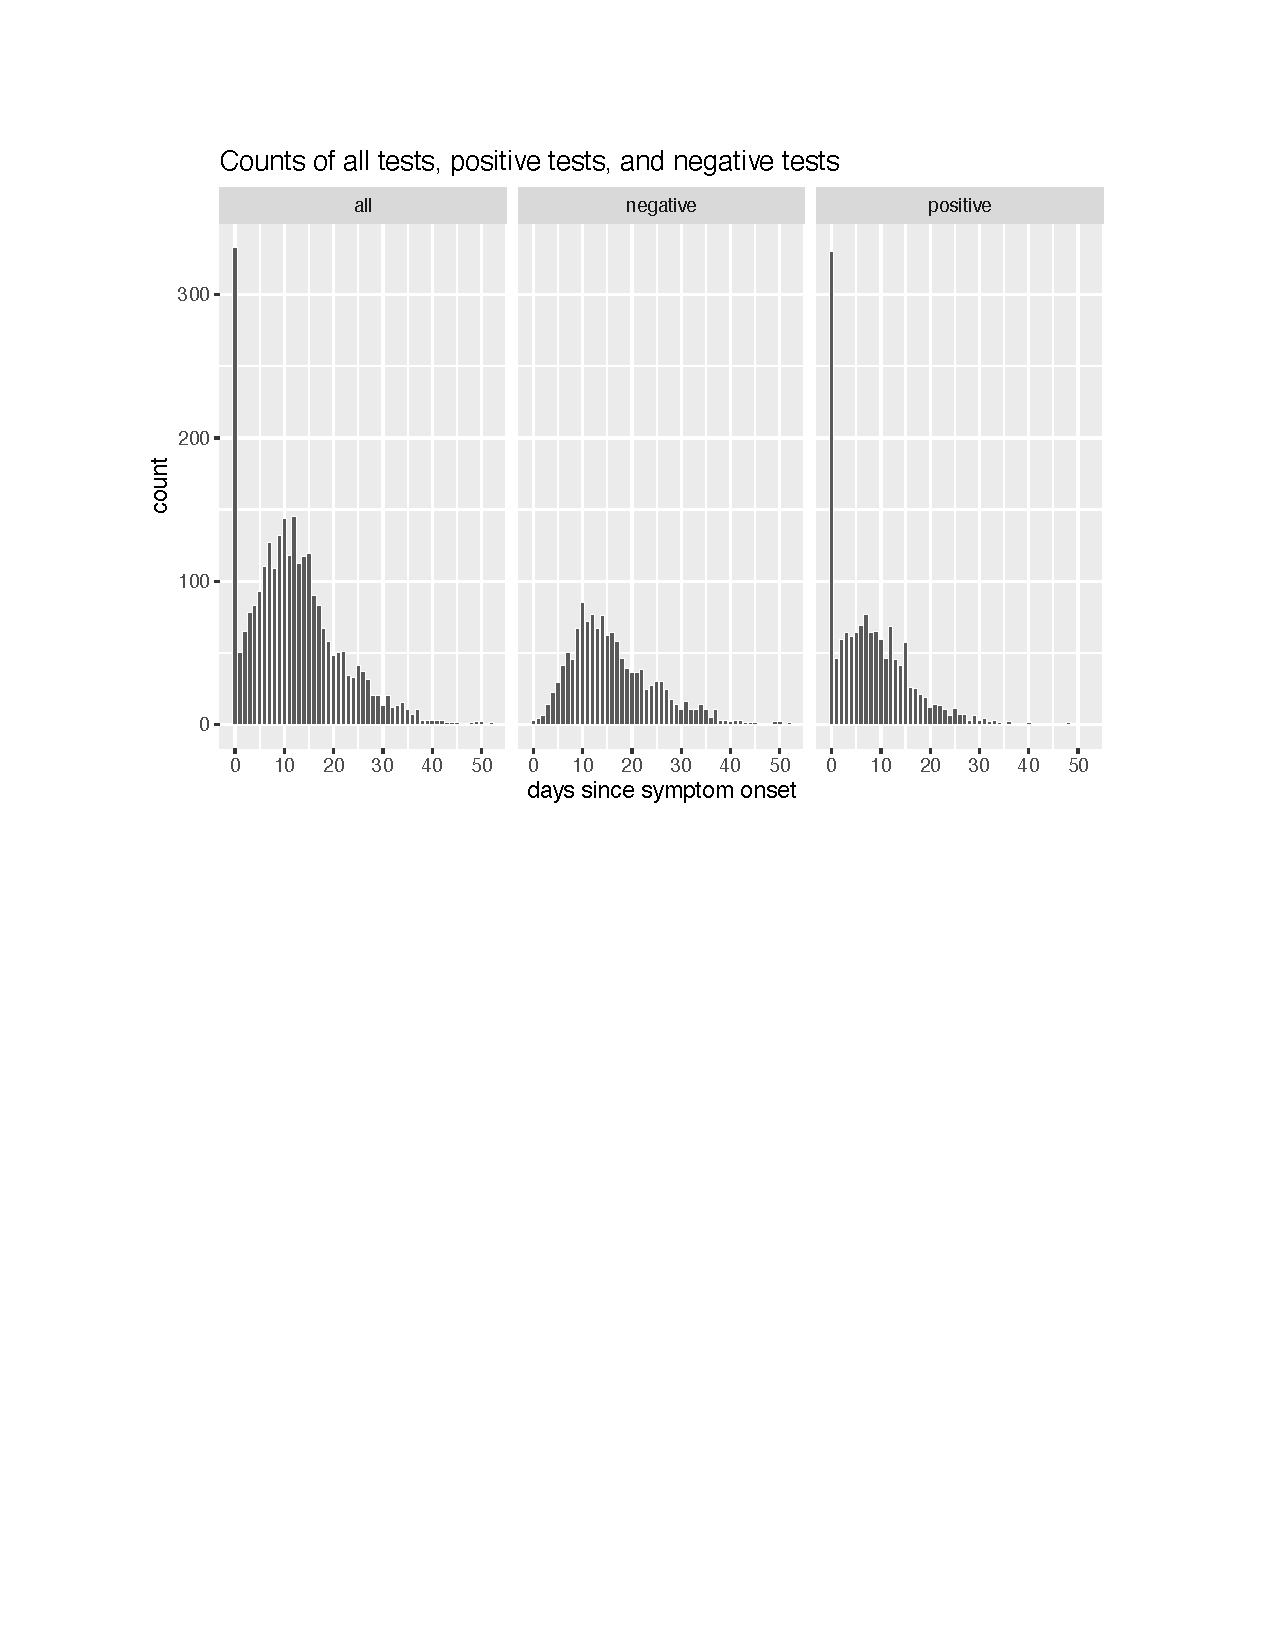
\includegraphics[width=0.8\textwidth]{img/test-pos-neg-counts.pdf}

\sld{Binomial MLE (days with tests)}

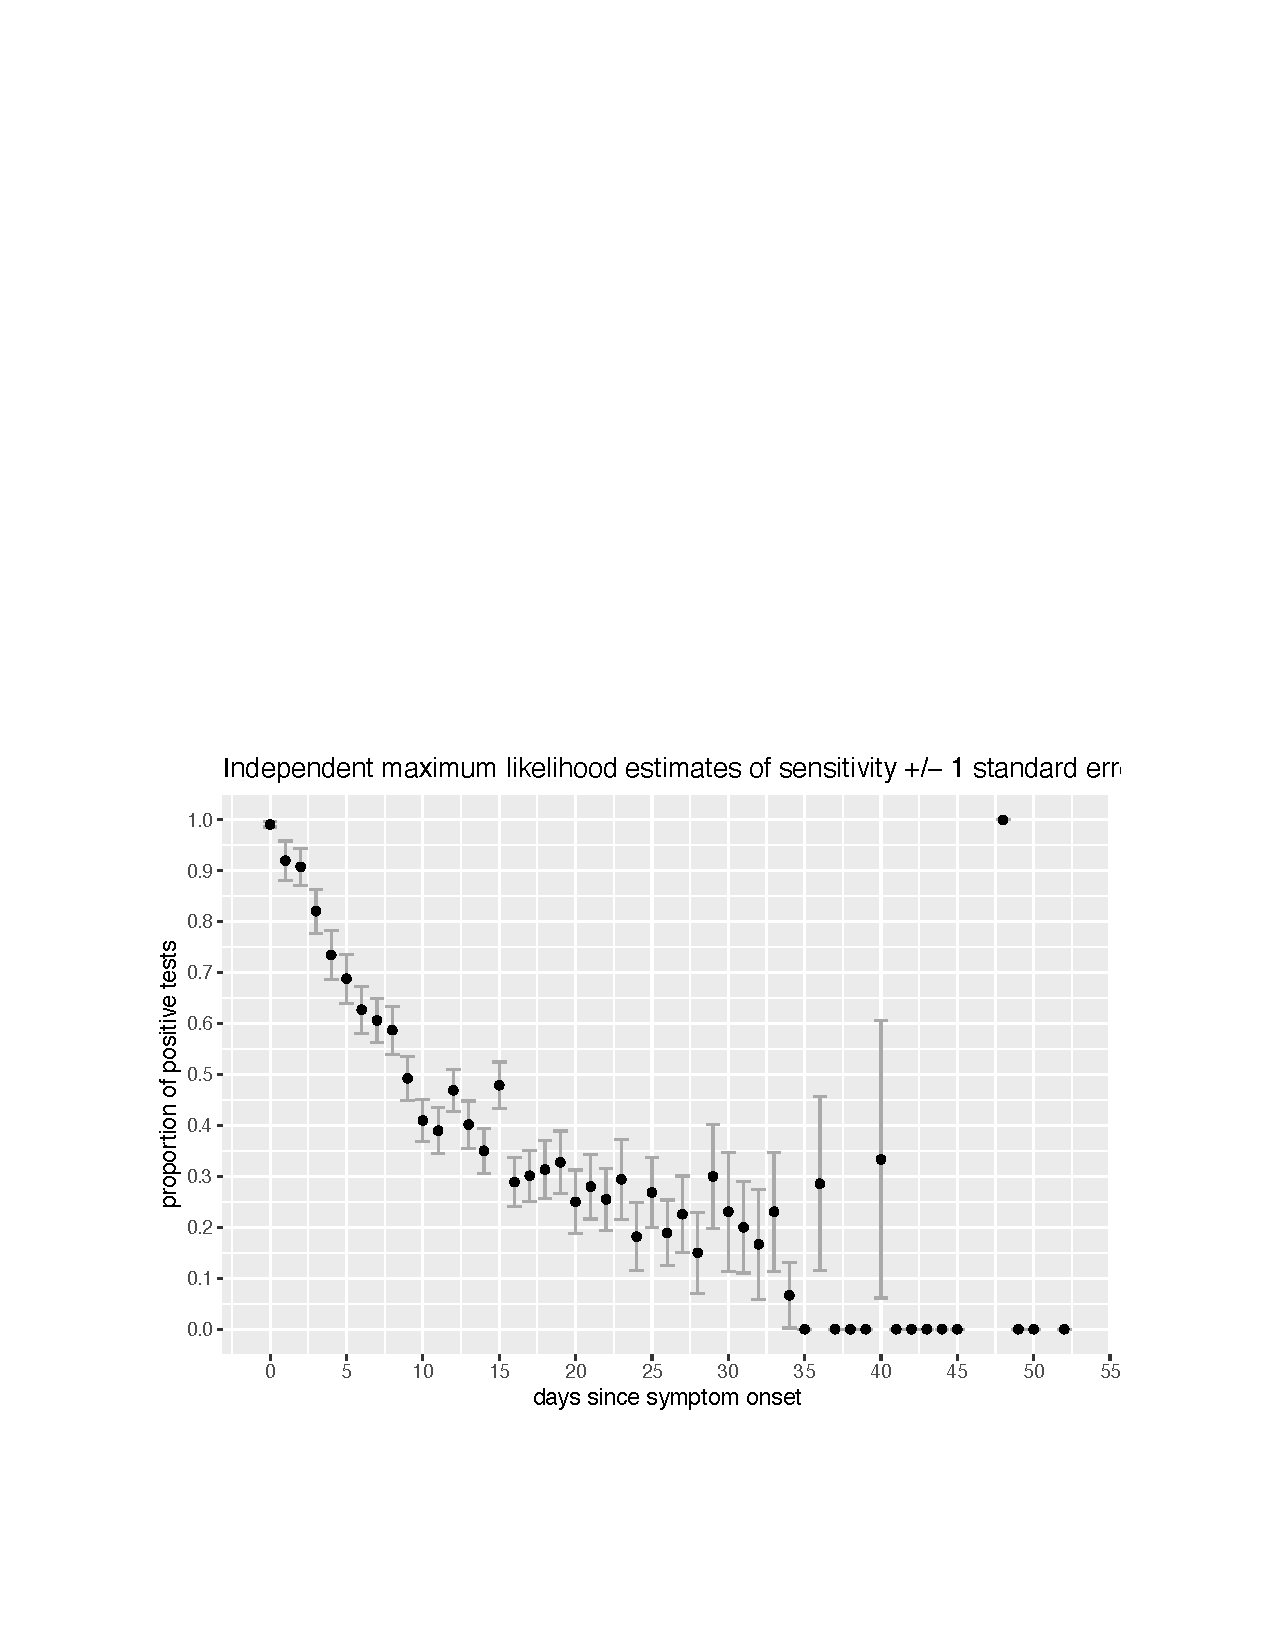
\includegraphics[width=0.75\textwidth]{img/mle-time-series.pdf}
\vspace*{-3pt}
\begin{subitemize}
  \item $y_t \sim \textrm{binomial}(N_t, \theta_t)$
  \end{subitemize}
  
\sld{Bayesian weakly informative}

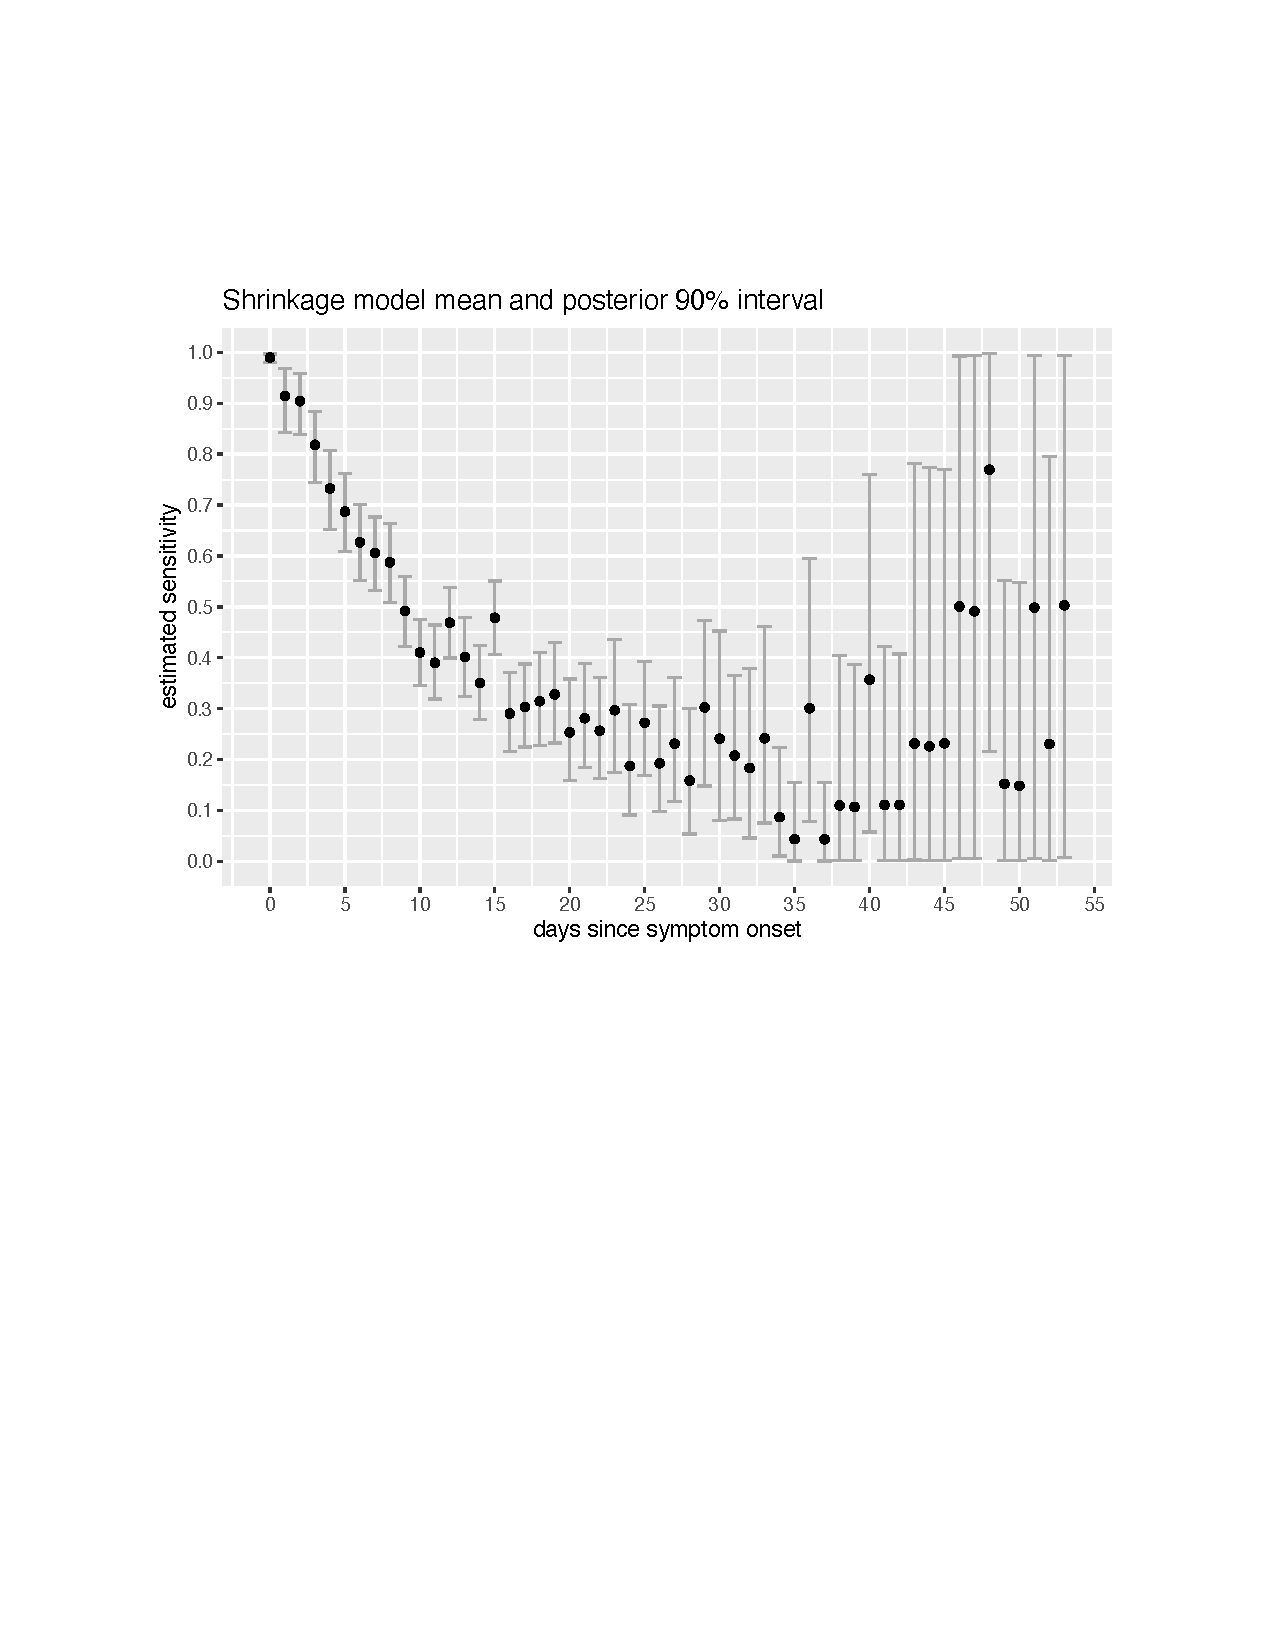
\includegraphics[width=0.75\textwidth]{img/bayes-90pct-shrinkage.pdf}
\vspace*{-3pt}
\begin{subitemize}
\item $\textrm{logit}(\theta_t) \sim \textrm{normal}(0, 3)$
\end{subitemize}

\sld{Bayesian with monotonicity}

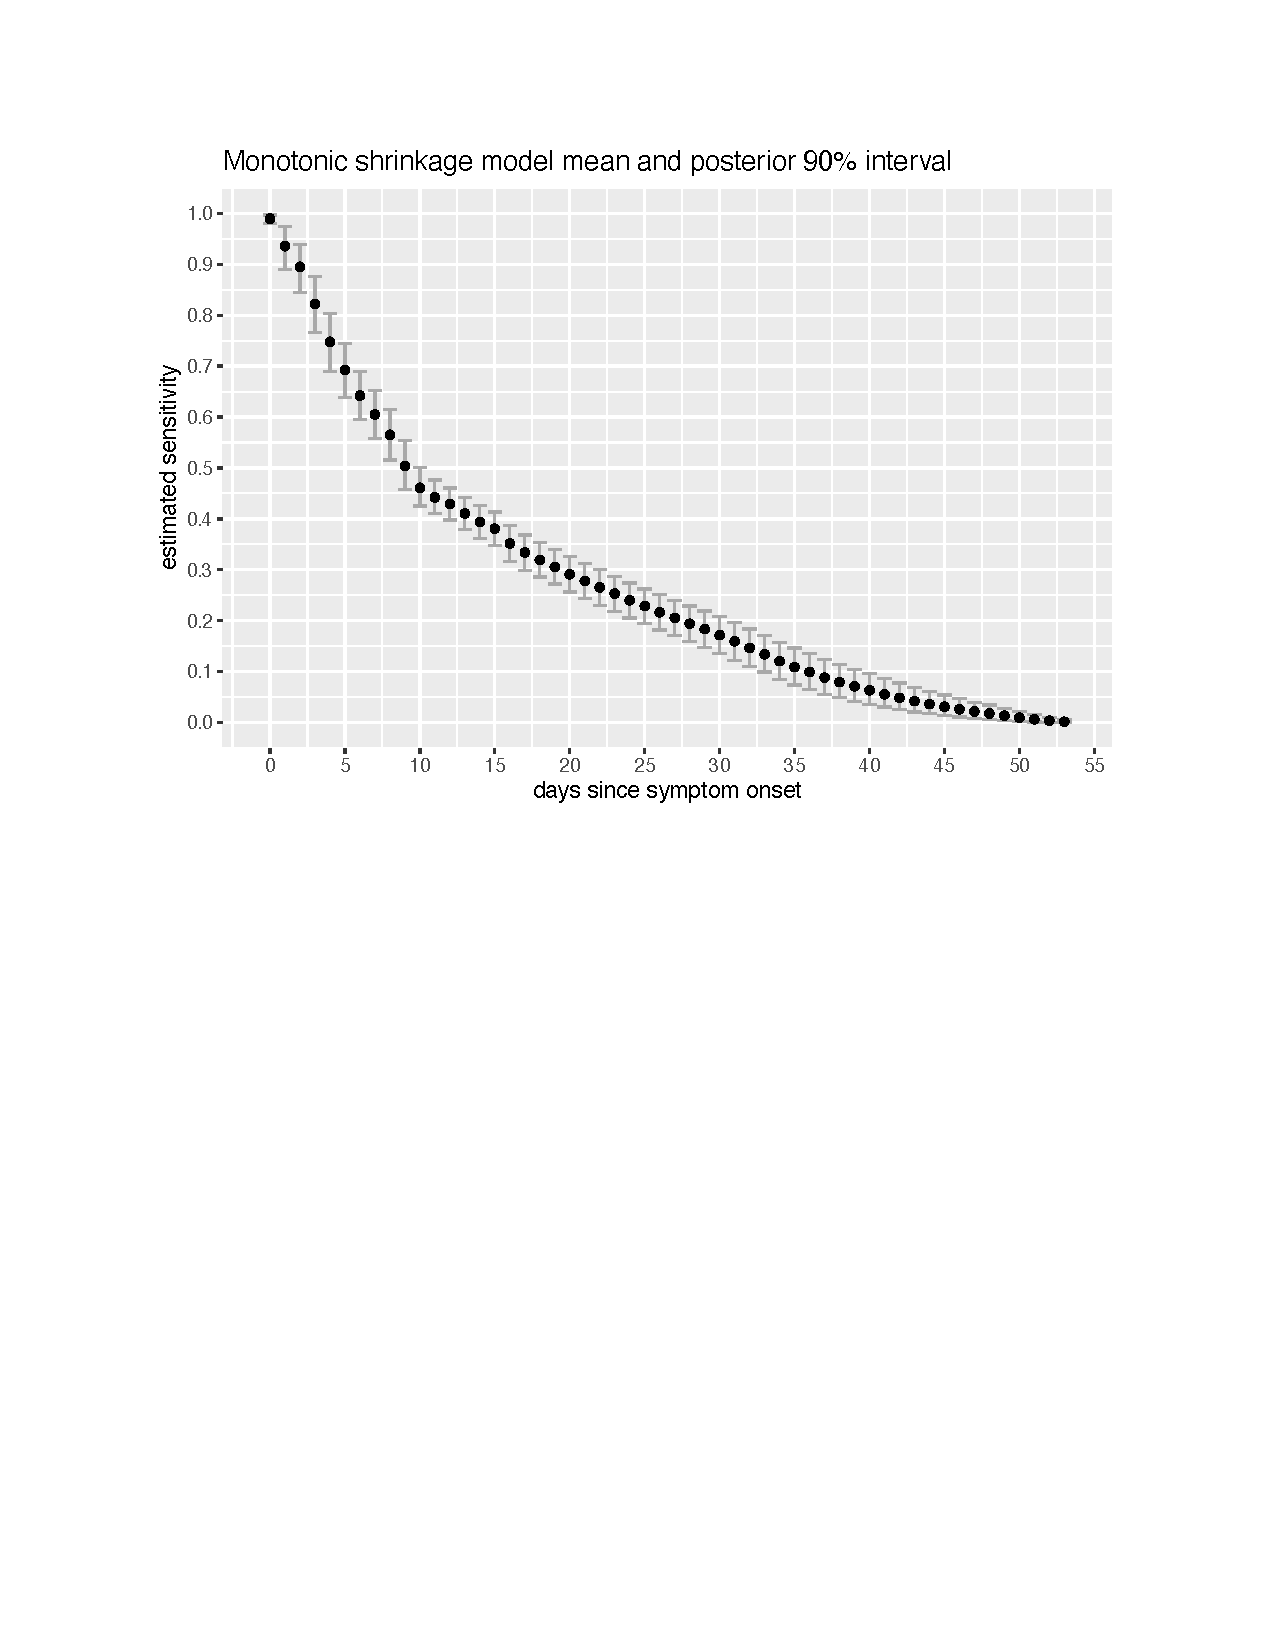
\includegraphics[width=0.7\textwidth]{img/monotonicity-bayes.pdf}
\vspace*{-3pt}
\begin{subitemize}
\item $\textrm{logit}(\theta_t) \sim \textrm{normal}(0, 3) \
  \textrm{s.t.} \ \theta_t > \theta_{t+1}$
\item \myemph{reduced uncertainty} due to \myemph{constraint}
\end{subitemize}

\sld{Bayesian 1st-order random walk}
  
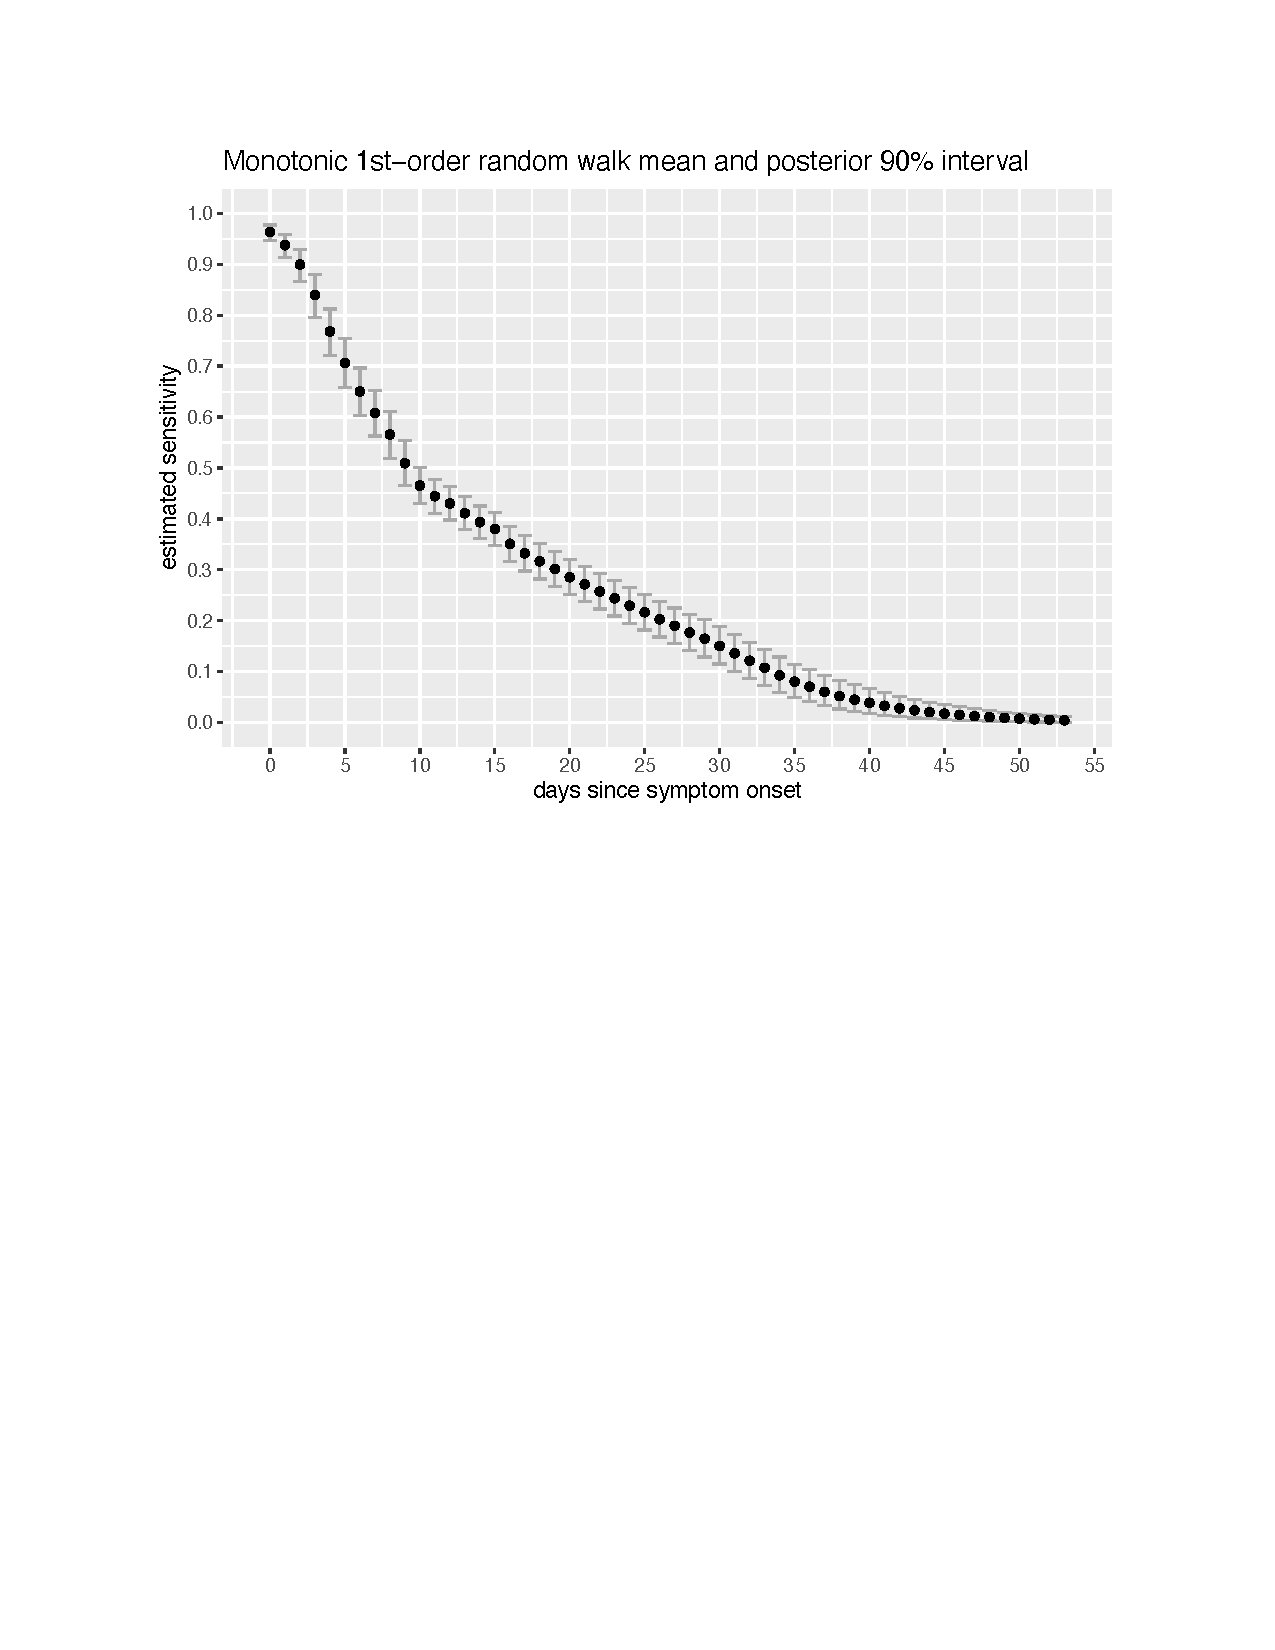
\includegraphics[width=0.7\textwidth]{img/monotonic-bayes-rw1.pdf}
\vspace*{-3pt}
\begin{subitemize}
\item $\textrm{logit}(\theta_{t+1}) \sim \textrm{normal}(\theta_{t-1}, 
  \sigma) 
  \quad \textrm{logit}(\theta_1) \sim \textrm{normal}(4, 1)$
  \\
  $\sigma \sim \textrm{normal}_+(0, 1)$
\end{subitemize}

\sld{Bayesian 2nd-order random walk}
  
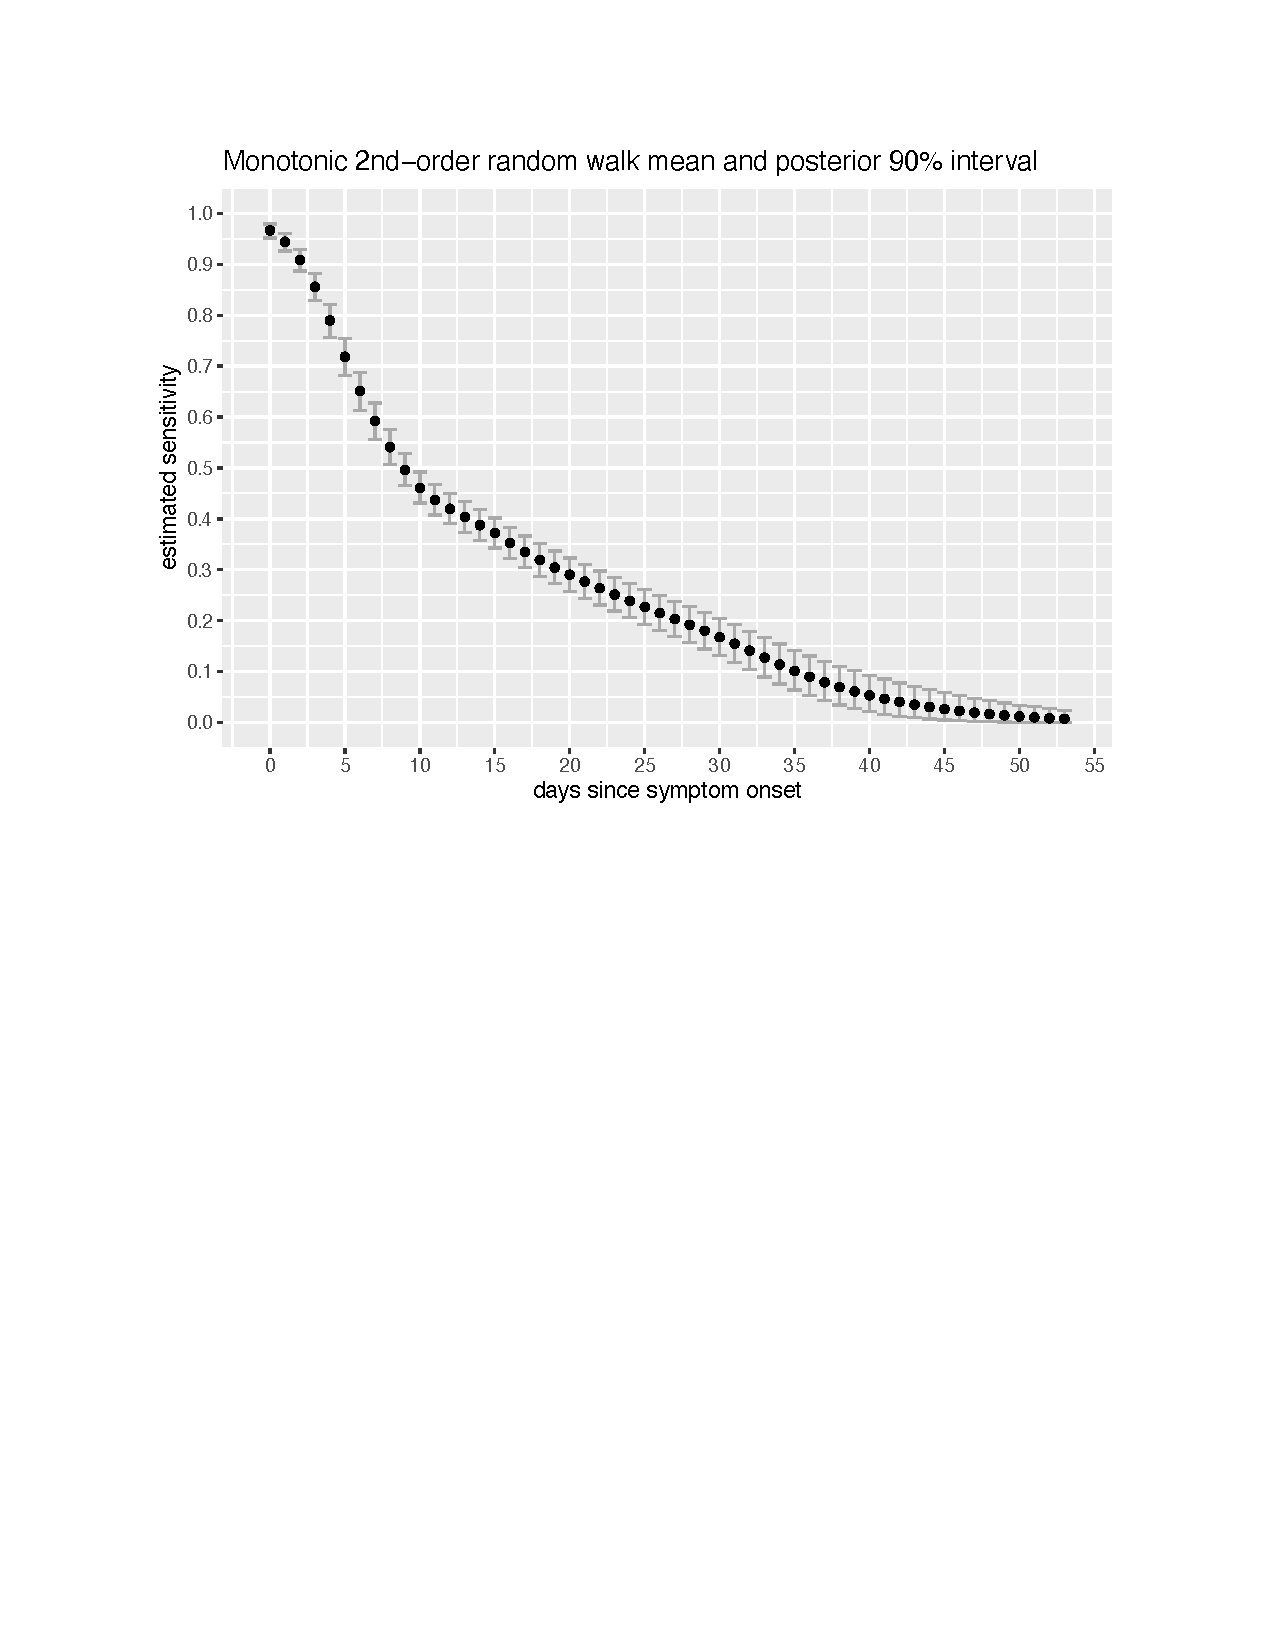
\includegraphics[width=0.7\textwidth]{img/mono-bayes-rw2.pdf}
\vspace*{-3pt}
\begin{subitemize}
\item $\textrm{logit}(\theta_{t+1}) \sim
  \textrm{normal}(\theta_{t-1} + (\theta_{t-1} - \theta_{t-2}),
  \sigma)$
  \\
  $\theta_2 \sim \textrm{normal}(\theta_1, 2\sigma)
  \qquad
  \textrm{normal}_+(0, 1)$
\end{subitemize}


\sld{Binomial GLM, logit link}
  
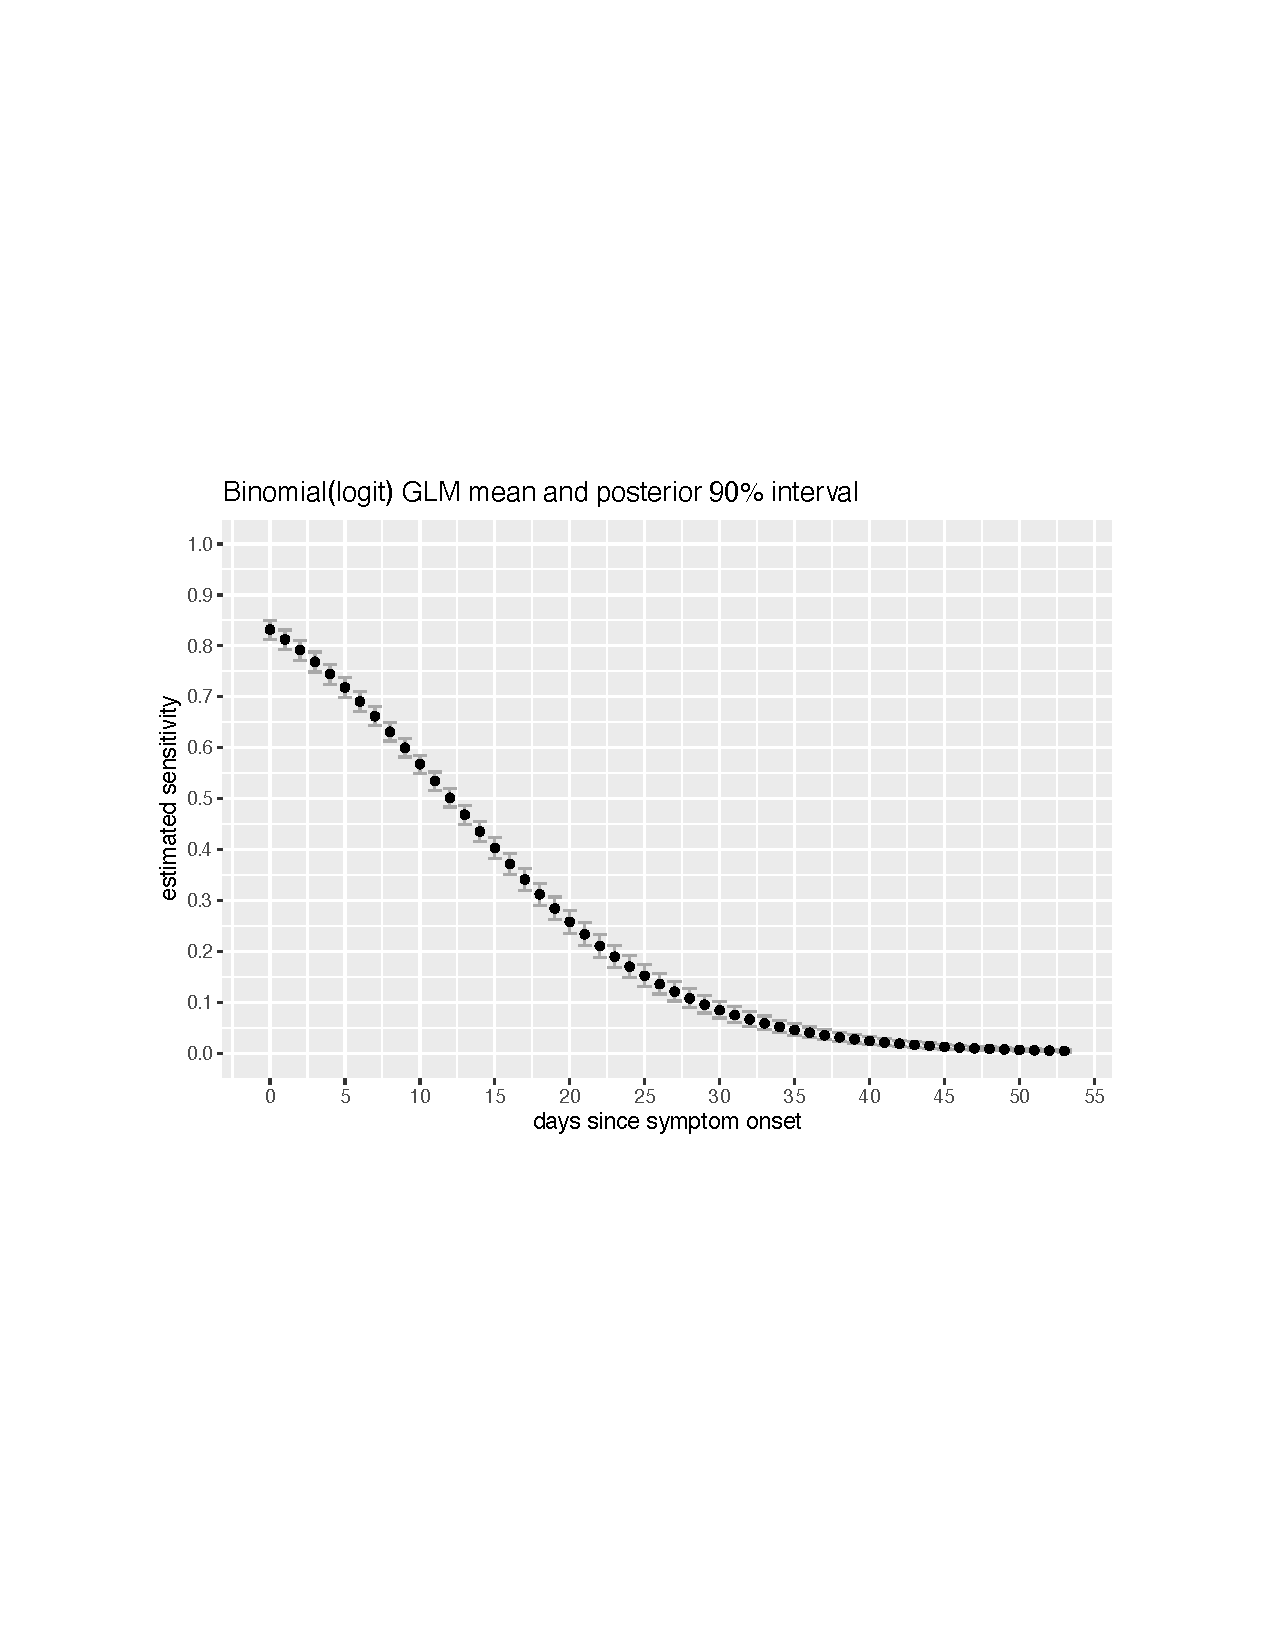
\includegraphics[width=0.7\textwidth]{img/bayes-logit-glm.pdf}
\vspace*{-3pt}
\begin{subitemize}
\item $y_t \sim \textrm{binomial}\left(N_t, \, \textrm{logit}^{-1}(\alpha +
  \beta \cdot t)\right)
  \quad \alpha, \beta \sim \textrm{normal}(0, 0.5)$
\item \myemph{very poor fit} in early days \myemph{forced by link}
\end{subitemize}


\sld{Binomial GLM, log link}
  
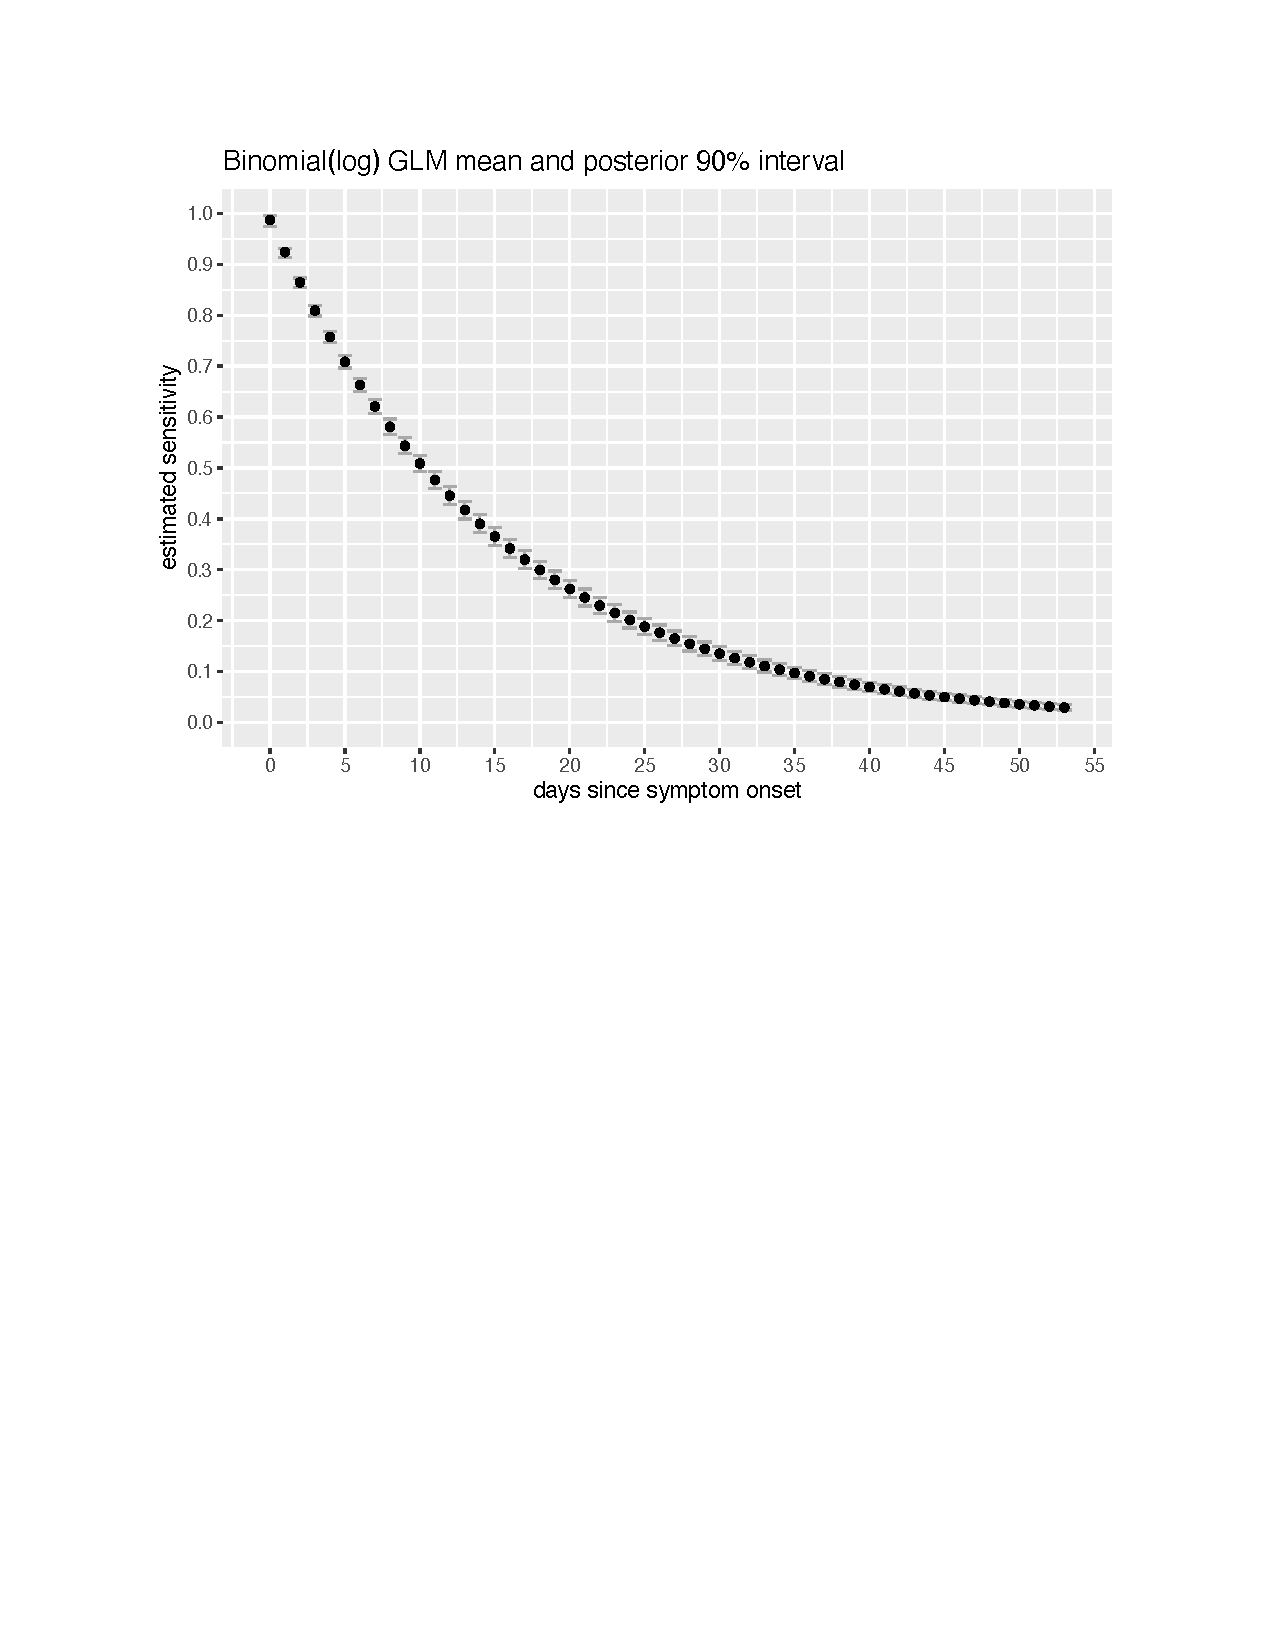
\includegraphics[width=0.7\textwidth]{img/bayes-binomial-log.pdf}
\vspace*{-3pt}
\begin{subitemize}
\item $y_t \sim \textrm{binomial}\left(N_t, \, \textrm{exp}(\alpha +
  \beta \cdot t)\right)
\quad \alpha, \beta \sim \textrm{normal}_(0, 0.5)$
\item $\alpha, \beta < 0$ enforces $\textrm{exp}(\alpha + \beta \cdot
  t) \in (0, 1)$
\end{subitemize}

\sld{Posterior for binomial-log}

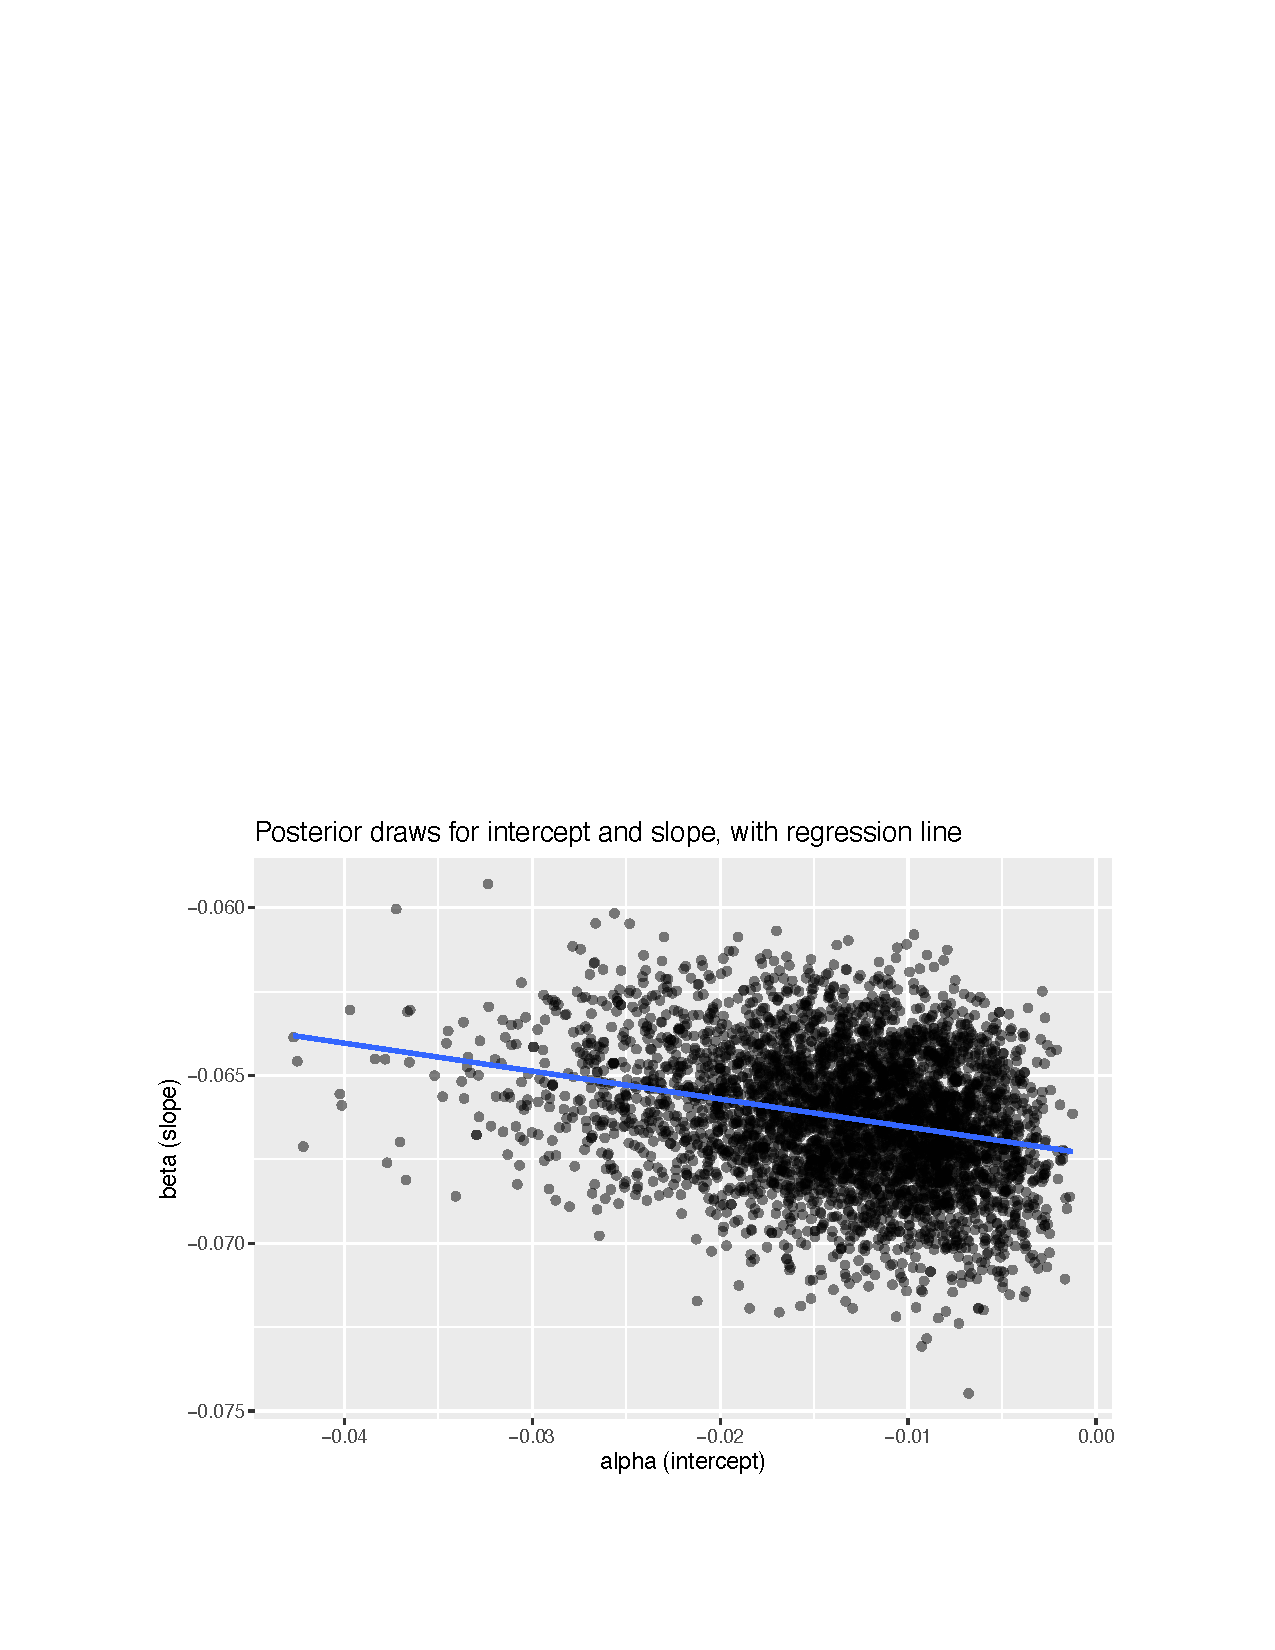
\includegraphics[width=0.7\textwidth]{img/binomial-log-scatter.pdf}
\begin{subitemize}
\item negative correlation because $t \geq 0$
\item intercept not well identified
\end{subitemize}

\sld{Leave-one out X-validation}

\vspace*{8pt}

\includegraphics[width=0.7\textwidth]{img/loo.pdf}
\vspace*{-3pt}
\begin{itemize}
\item \myemph{ELPD}: expected log \myemph{pointwise predictive} density
  \begin{subitemize}
  \item estimated with \texttt{\bfseries loo} package in R
  \item based thousands of observations (cf. earlier histograms)
  \end{subitemize}
\item \myemph{binary outcome} probabilities \myemph{hard to discriminate}
\end{itemize}
  
\sld{Interpreting the results (1)}
\begin{itemize}
\item \myemph{best}: binomial log (left) \& monotonic shrinkage (right)
  \begin{subitemize}
  \item \myemph{cannot discriminate} with this data
  \item actual fits look very different
  \end{subitemize}
\end{itemize}
\begin{center}
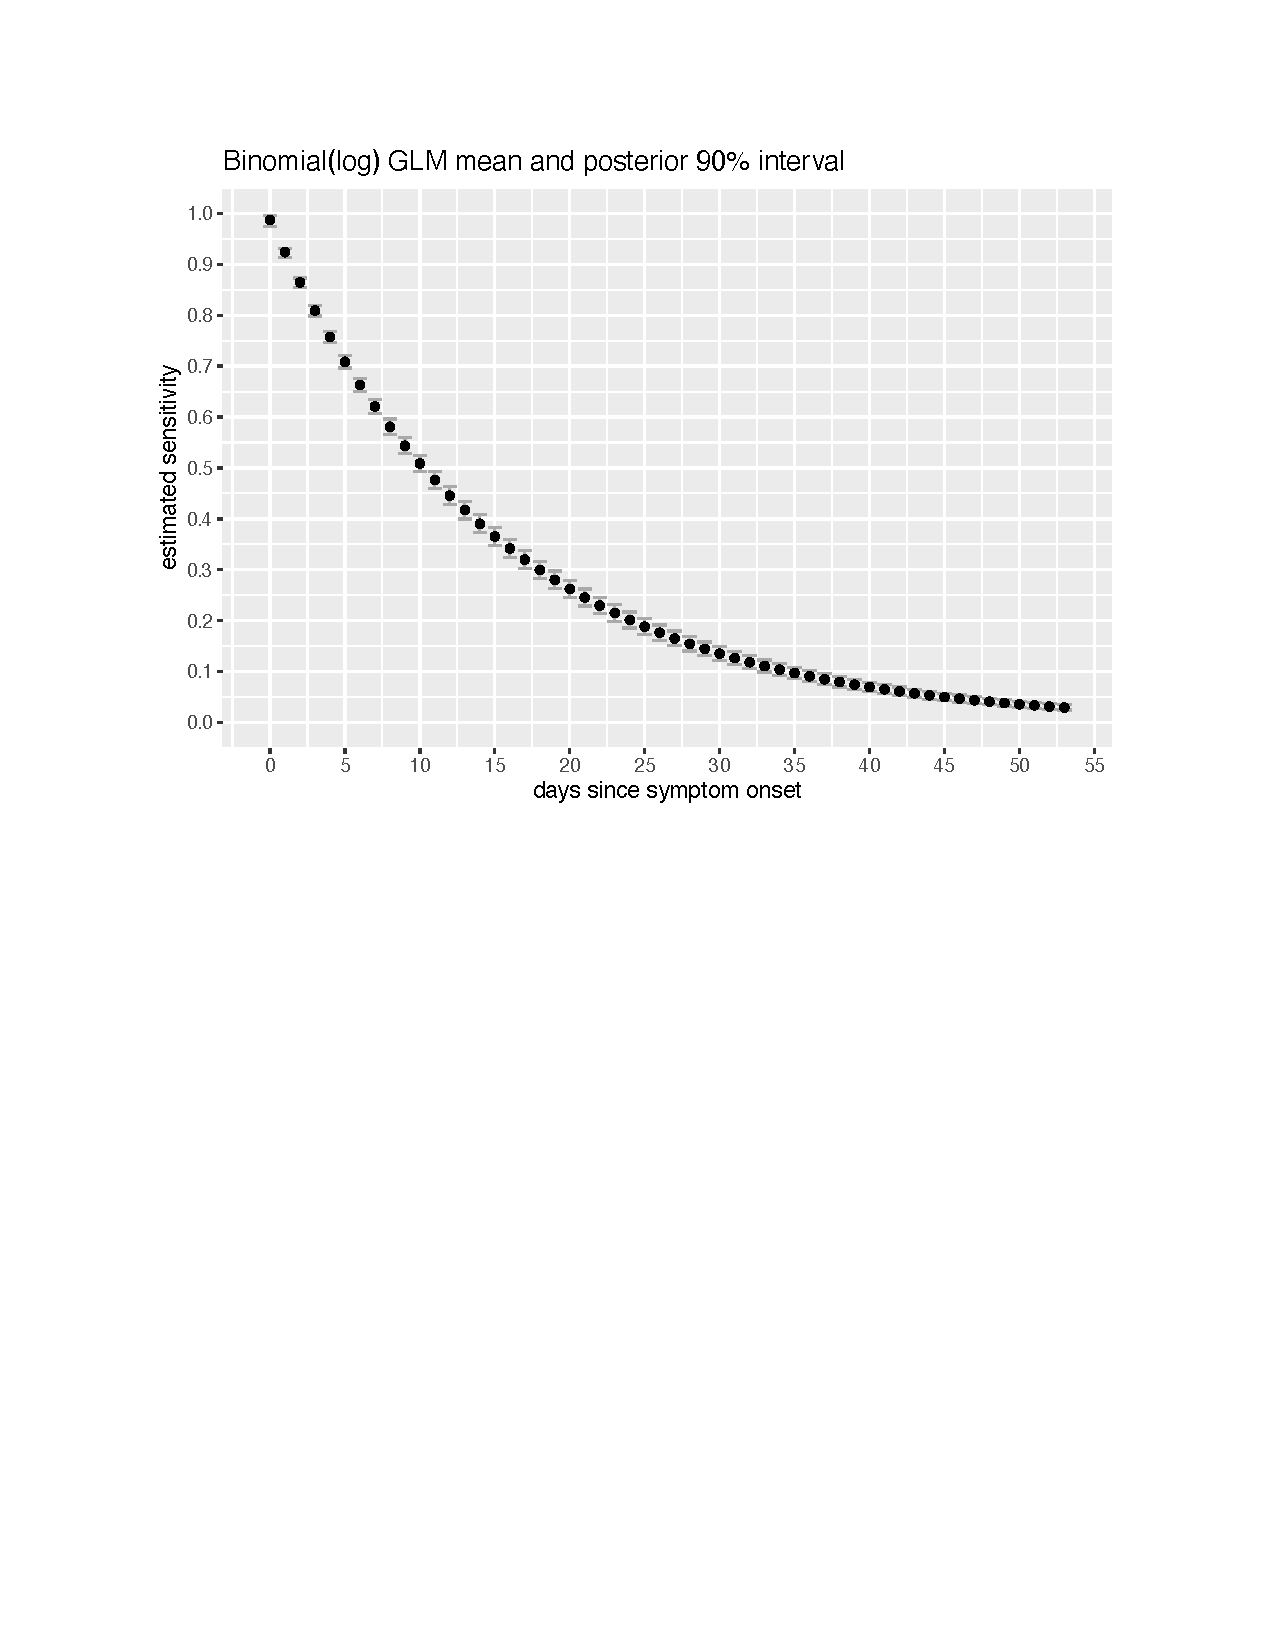
\includegraphics[width=0.45\textwidth]{img/bayes-binomial-log.pdf}
\quad
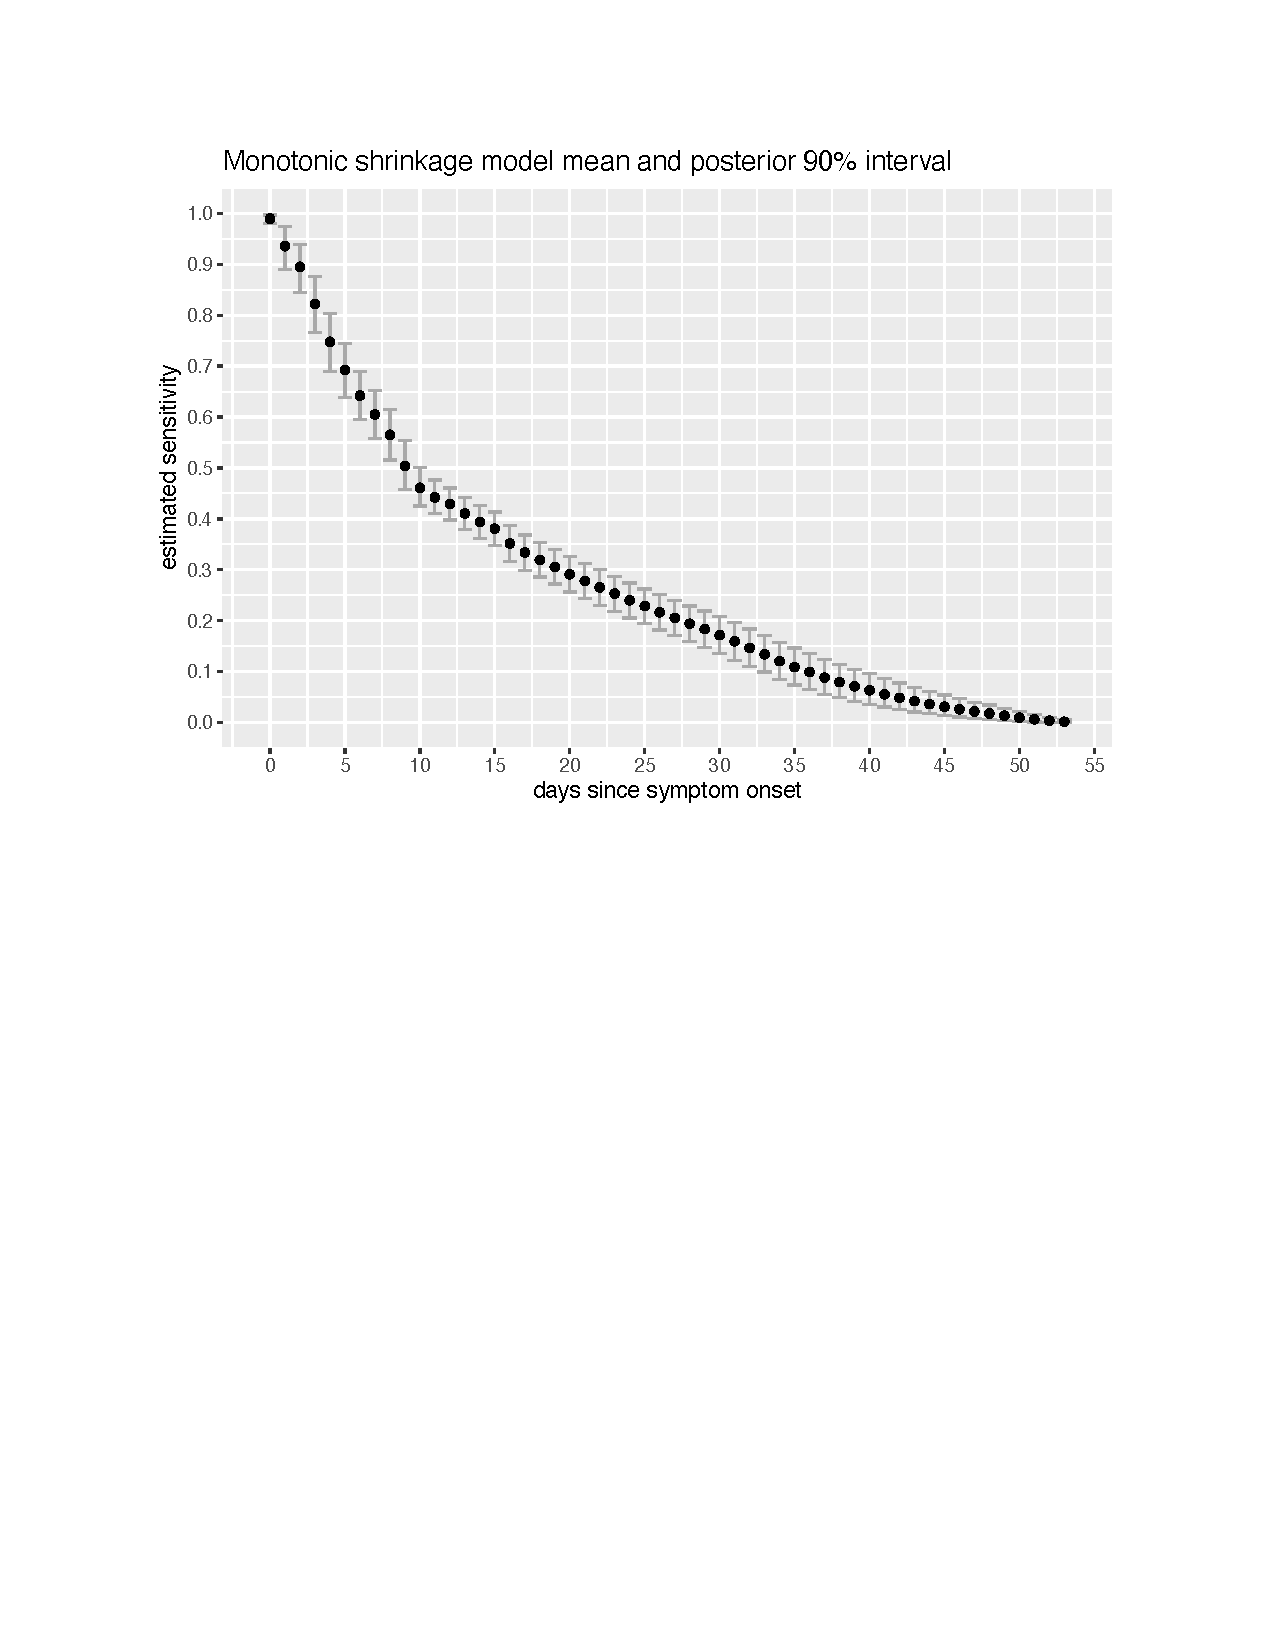
\includegraphics[width=0.45\textwidth]{img/monotonicity-bayes.pdf}
\end{center}


\sld{Interpreting the results (2)}
\begin{itemize}
\item \myemph{binomial GLM}
  \begin{subitemize}
  \item 2 parameters
  \item strong assumptions: link models \myemph{exponential clearance}
  \item parameters not well identified, but sensitivity at time is
  \end{subitemize}
\item \myemph{monotonicity constraint} with weakly informative prior
  \begin{subitemize}
    \item flexible \myemph{non-parametric} model (parameter per time)
    \item e.g., can \myemph{fit mixture} of long- and short-covid (cf. kink
      at 10 days)
    \item wider posterior intervals on test sensitivity
    \end{subitemize}
\end{itemize}

\sld{Caveats}
\begin{itemize}
\item data is from \myemph{hospitalized} patients
  \begin{subitemize}
  \item many stay in hospital due to \myemph{long Covid}
  \item \myemph{not representative} of general population
  \end{subitemize}
\item as many as 10 tests per patient
  \begin{subitemize}
  \item but \myemph{within-patient effects} not modeled
  \end{subitemize}
\end{itemize}

\sld{\vspace*{-4pt}Professional basketballer data}

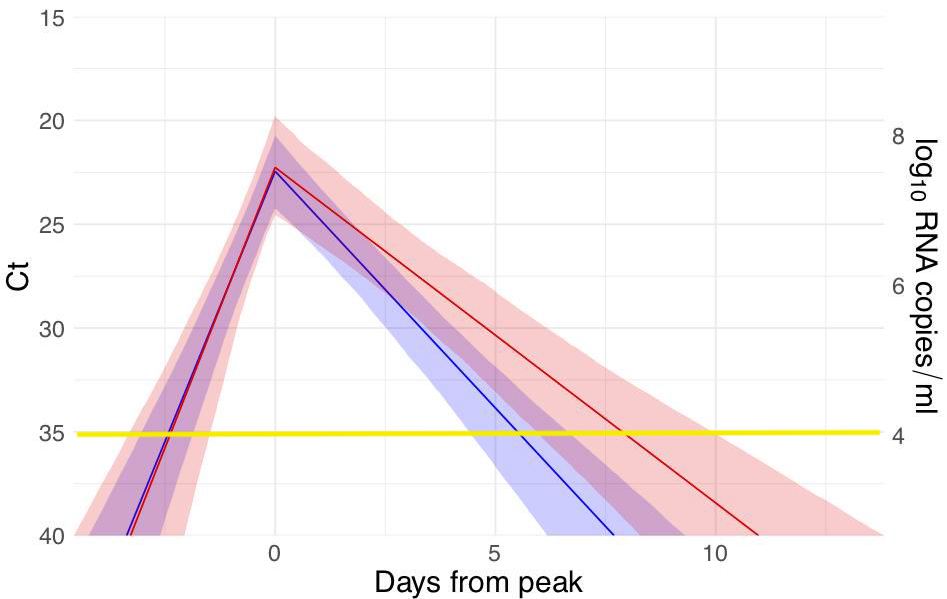
\includegraphics[width=0.7\textwidth]{img/bball-days-from-peak.png}
\begin{subitemize}
\vspace*{-4pt}
\item all \myemph{tested positive}; 
\myemph{symptomatic} red; \ \myemph{asymptomatic} blue
\vspace*{-4pt}
\item PCR tests \myemph{only sensitive} at $\textrm{Ct} < 35$ for $t \in (-5, 10)$
\vspace*{-4pt}
\item \footnotesize Kissler et al. 2021. Viral dynamics of acute
  SARS-CoV-2 infection and applications to diagnostic and public
  health strategies. \textit{PLOS Bio.}
\end{subitemize}


\sld{UK tests vs.\ deaths}

\begin{itemize}
\item (1) tens of millions of voluntary tests
\item (2, 3) UK \myemph{national ``surveys''} (ONS/Oxford \& NHS/UCL)
\item strong \myemph{positive opt-in biases} \& \myemph{no agreement}
\item even after \myemph{post-stratification} for \myemph{demographic
    biases}
  \vfill
\item \myemph{Covid deaths} are more reliable measure
  \begin{subitemize}
  \item still require distinguishing \myemph{dying with}
    vs. \myemph{dying of} Covid
  \item \myemph{criteria vary by region} \& \myemph{changed} mid-pandemic
  \end{subitemize}
\end{itemize}

\sld{Time to death model}
\begin{itemize}
\item UK Health Security Agency fit \myemph{time-to-death} model
  \begin{subitemize}
  \item all conditioned on patient dying of Covid
  \end{subitemize}
\item \myemph{continuous} $\textrm{lognormal}(\mu^d, \sigma^d)$ best
  fits distribution
\item but we need \myemph{discrete} probability of \myemph{death by day}:
  \\[8pt]
  $\textrm{Pr}[\textsf{\small die during day } t \mid \mu^d, \sigma^d]$
  \\[4pt]
  ${} = \textrm{Pr}[\textsf{\small die before day } t + 1 \mid \mu^d,
  \sigma^d]$
  \\[4pt]
  ${} \quad  - \textrm{Pr}[\textsf{\small die before day } t \mid \mu^d, \sigma^d]$
\end{itemize}

\sld{Infection fatality rate}
\begin{itemize}
\item use estimate of \myemph{infection fatality rate}
  \begin{subitemize}
  \item probability of dying given infected with Covid
  \item obviously varies tremendously by demographics
  \item shortened as hospitals were overwhelmed
  \end{subitemize}
\item we will use a \myemph{point estimate}
$$\widehat{\delta} \approx \textrm{Pr}[\textsf{\small patient dies} \mid
\textsf{\small patient Covid positive}]$$
\vspace*{-18pt}
\begin{subitemize}
\item it would be better to \myemph{propagate estimation uncertainty}
\end{subitemize}
\end{itemize}

\sld{Generative model of deaths}
\begin{itemize}
\item let $\theta_t \in (0, 1)$ be the \myemph{infection rate} on day $t$
\item $\widehat{\delta} \cdot \theta_t$ of those people expected
  to die
  \begin{subitemize}
  \item should include sampling variation
  \end{subitemize}
\item derive \myemph{expected deaths} on day $t+1, t+2, \ldots$
  \begin{subitemize}
  \item from infections on day $t$ with \myemph{time of death model}
  \end{subitemize}
\item derive \myemph{expected deaths} on day $t$
  \begin{subitemize}
  \item from expected deaths on $t-1, t-2, \ldots$ to
  \end{subitemize}
\item \myemph{Poisson} model of \myemph{observed deaths} given expected deaths
\item solve \myemph{inverse problem} with \myemph{Bayesian inference}
\end{itemize}

\sld{Estimate random testing results}
\begin{itemize}
\item death model yields \myemph{estimated infection rate} rate $\theta_t \in (0, 1)$ on
  day $t$
  \begin{subitemize}
  \item with some, but not all relevant uncertainty
  \end{subitemize}
\item for each day $t$, we know fraction of population estimated to
  have been \myemph{infected each previous day}
\item use test positivity to estimate \myemph{random testing positivity}
  \vfill
\item could potentially use to \myemph{adjust opt-in and survey biases}
\end{itemize}

\sld{Backcasting result}

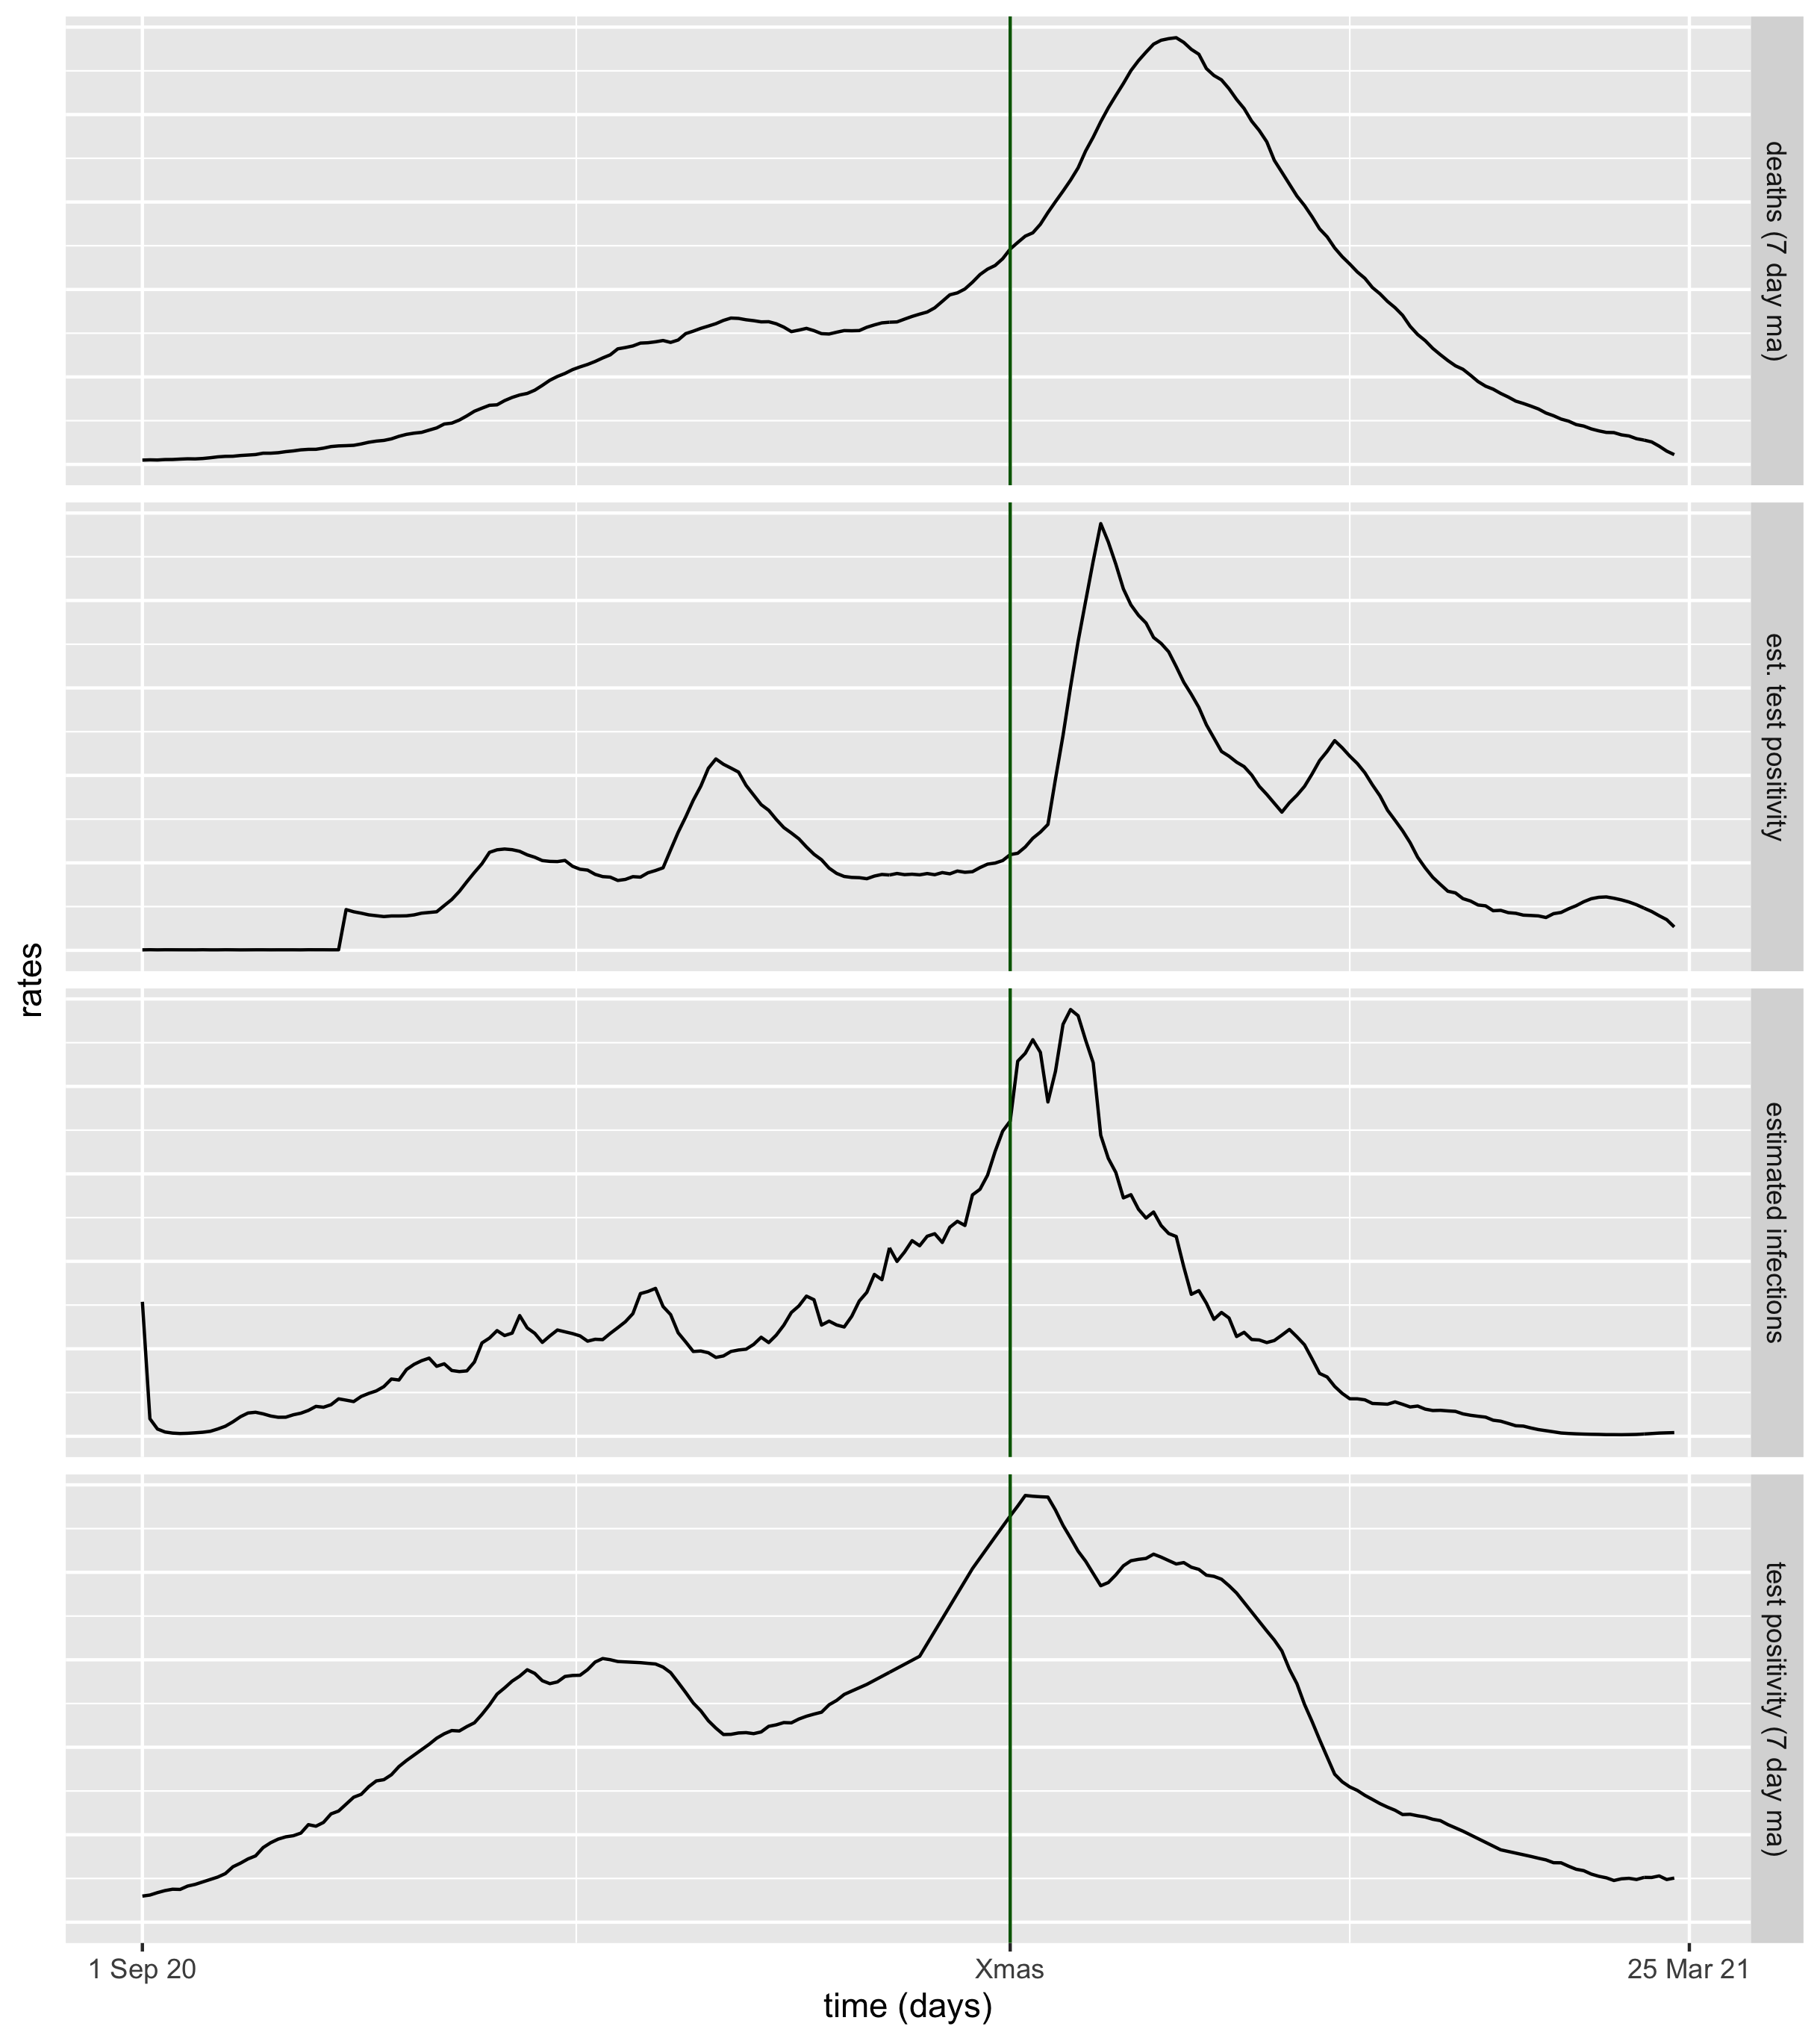
\includegraphics[height=0.9\textheight]{img/deaths-predict.png}
\quad 
\begin{minipage}[t]{1.5in}
  \vspace*{-2.2in}\footnotesize 
  (a) deaths, 7 day moving average 
  \\[18pt]
  (b) estimated random test positivity 
  \\[18pt]
  (c) estimated infections 
  \\[30pt]
  (d) actual test positivity 
  \\[8pt]
  \footnotesize (*) \myemph{x axis}: 1 Sep to 25 Mar, vertical at \myemph{Xmas 2020}
  \\ \myemph{y axis}: rates
\end{minipage}

\sld{Acknowledgements \& Code}

\begin{itemize}
\item \myemph{hierarchical model} joint work with \myemph{Andrew
    Gelman}
  \begin{subitemize}
    \item Gelman \& Carpenter. 2020. Bayesian analysis of tests with unknown specificity and sensitivity. \textit{JRSS C}.
  \end{subitemize}
\item \myemph{other models} joint work with \myemph{Tom Ward}
  \begin{subitemize}
    \item head of infectious disease modeling for UK Health
    Security Agency
    \end{subitemize}
\vfill
\item \myemph{Stan code} for hierarchical model in paper (and GitHub)
\item other code on GitHub: \texttt{\bfseries bob-carpenter/epi-mrp}
  \begin{itemize}
  \item lots of fiddly indexing and marginalizations
  \end{itemize}
\end{itemize}


\end{document}


